\chapter{Where the app stands today: the builds}\label{ch:builds}

\lead{The earlier chapters describe what the code is meant to do. This chapter looks at what it has actually produced. It covers the archive of every run output that existed on 5 November 2026, the representative figures taken from it, nine build cards, a command-line run made on the current working tree the same day, and the defects these outputs expose.}

Every number in this chapter comes from one of three sources. The first is the archive index \code{builds/_archive_2026-11-05/BUILDS_ARCHIVE_INDEX.md} and its machine-readable twin \code{catalog.json}, both generated by a read-only walk of the old \code{builds/} tree. The second is the per-build records: \code{summary.json}, \code{metadata.txt} and the images. The third is the logs and \code{summary.json} of a fresh run on the working tree, kept outside the repository.

None of the results is physically validated, and the chapter uses the repository's own maturity labels. Every build that records the \code{hardware_qualified} flag records \code{False}. The label \code{rao_variational_residual_solved} on the variational contours is a statement about numerical closure, and the chart-based contours carry the design status \code{preliminary_top_geometry}. The newer summaries list 17 missing external-evidence items, among them computational fluid dynamics (CFD), conjugate heat transfer (CHT), finite-element analysis (FEA), cold flow and hot fire, and report the physical release as blocked.

%======================================================================
\section{The builds archive}\label{sec:builds-archive}

\subsection{What was archived}\label{sec:builds-archive-what}

On 5 November 2026 every build in the repository was moved intact into \code{builds/_archive_2026-11-05/}. Nothing was deleted or rewritten. The archive holds 523 top-level entries: 522 from \code{builds/} and one stray copy from \code{scripts/builds/}. Together they contain 1931 files and 1,704,308,042 bytes (1.6\,GB). By kind there are 454 versioned \code{vNNN_<timestamp>} directories, 47 named directories, 20 loose files, one \code{samples/} folder and one \code{tests/} folder, which holds six sub-builds.

STL meshes account for 1.2\,GB of the total, STEP files for 250.9\,MB, PNG images for 57.9\,MB and GIF animations for 31.7\,MB. All the CSV contours together come to 5.2\,MB. By file count the order is CSV 520, text 452, PNG 419, STL 198, STEP 148 and JSON 142.

After the move, \code{builds/} holds a short \code{README.md} and a placeholder directory, \code{builds/v454_archived_20261105/}. The placeholder is needed because \code{raosim.build_log._next_version()} (\code{raosim/build_log.py:25}) numbers new builds by scanning \code{builds/} for the highest \code{vNNN_} prefix, so without it new builds would start again at v001.

Table~\ref{tab:builds-families} lists the 18 families that the index assigns.

{\footnotesize
\newcolumntype{N}[1]{>{\raggedleft\arraybackslash}p{#1}}
\begin{longtable}{P{3.25cm}N{1.0cm}N{0.8cm}N{1.35cm}P{2.05cm}P{6.35cm}}
\caption{Build families in the archive. The figures are taken from \texttt{BUILDS\_ARCHIVE\_INDEX.md} section 2. Dates are in 2026 and are the newest-file dates of each family's entries. The exception is tests-products, whose six sub-builds carry files dated 2 to 17 July.}\label{tab:builds-families}\\
\toprule
Family & Entries & Files & Size & Dates & Content\\
\midrule
\endfirsthead
\toprule
Family & Entries & Files & Size & Dates & Content\\
\midrule
\endhead
\bottomrule
\endfoot
versioned-cli-contour & 436 & 872 & 5.2 MB & 05-11 to 10-16 & Legacy \code{main.py} batch runs writing \code{cli_bezier.csv}, \code{cli_moc.csv} or \code{cli_rao.csv} with a design-gates block; long runs of byte-identical output\\
13kn-engine-package & 14 & 366 & 551.6 MB & 06-28 to 06-30 & 13\,kN LOX/RP-1 packages: contour, wall and jacket STL/STEP, regen, pintle, \code{pump.json}; 316L, GRCop-84/Inconel 718, flanged, 20 and 40\,bar variants; \code{lrekit_*} benchmarks, \code{complete_seed}, \code{13kn_engine}, the stray \code{scripts/builds} copy\\
tests-products & 1 & 243 & 235.3 MB & 07-02 to 07-17 & \code{builds/tests/}: sea-level fast and full runs, rao-bvp flow field, the 13 July sandbox evaluation, the coaxial injector\\
cli-mode-demos & 11 & 60 & 183.2 MB & 06-15 to 06-17 & \code{run_*} demonstrations of CLI modes (smoke, interactive, show/no-show, flow field, animation, sized/auto-size)\\
nozzle-run-regen & 10 & 109 & 272.6 MB & 06-17 to 06-30 & \code{nozzle_run*} trees with regen, cooling and structural plots; four directories are empty\\
visual-joyride & 4 & 39 & 86.4 MB & 06-19 & Regen-channel and B-rep visual experiments (methane helix runs, $R_t = 50$\,mm, $\varepsilon = 8.5$)\\
pintle-injector-bundles & 6 & 116 & 73.6 MB & 06-29 & Pintle bundles for Inventor hand-off and the machined-pintle review before and after fixes\\
versioned-cli-smoke & 3 & 8 & 69.4 MB & 05-11 to 06-14 & Smoke runs; v019 carries a 72.7\,MB \code{rao_nozzle.step}\\
loose-nozzle-renders & 8 & 8 & 64.1 MB & 06-15 to 06-17 & Loose \code{regen_nozzle_*} STL/PNG and flow-field PNGs\\
samples-products & 1 & 44 & 52.8 MB & 06-30 & \code{samples/latest_13kn_check}, a complete 13\,kN package including pump\\
versioned-interactive & 8 & 19 & 23.8 MB & 03-06 to 06-28 & Interactive runs with typed output names (\code{whatever}, \code{take2}, \code{stuff}, \code{bro}, \dots)\\
versioned-early-batch & 3 & 8 & 3.7 MB & 03-02 to 03-09 & First Rao-bell runs; \code{rao_nozzle_profile.csv} only, no gates\\
versioned-no-metadata & 2 & 2 & 1.8 MB & 03-08 to 05-11 & Version folders with one file and no \code{metadata.txt}\\
loose-animation-frames & 4 & 4 & 837.8 KB & 06-17 & MOC-march and particle GIFs and their frame PNGs\\
rao-domain-scans & 2 & 12 & 486.3 KB & 08-24 to 08-26 & Rao chart-domain existence scans (Section~\ref{sec:build-cards})\\
versioned-batch-v2 & 2 & 6 & 327.4 KB & 05-14 to 06-20 & Two batch-v2 runs that also wrote \code{design_report_v2.json}\\
cea-tables & 1 & 8 & 188.4 KB & 08-22 & Frozen-chemistry CEA lookup tables (\code{.npz}) with validation JSON for four propellant pairs\\
loose-research-probes & 7 & 7 & 130.7 KB & 06-11 to 06-12 & J4/J5 and $\theta_B$ research probes\\
\midrule
\textbf{Total} & \textbf{523} & \textbf{1931} & \textbf{1.6 GB} & 03-02 to 10-16 & \\
\end{longtable}
}

\subsection{Timeline}\label{sec:builds-archive-timeline}

Table~\ref{tab:builds-timeline} groups the 523 entries by the month of each entry's newest file, using the timestamps recorded in \code{catalog.json}. The versioned count is the per-month total that the index reports for the \code{vNNN} series.

{\footnotesize
\newcolumntype{N}[1]{>{\raggedleft\arraybackslash}p{#1}}
\begin{longtable}{P{1.55cm}N{1.15cm}N{0.9cm}N{1.5cm}N{1.15cm}P{8.55cm}}
\caption{Archive timeline by month (2026).}\label{tab:builds-timeline}\\
\toprule
Month & Entries & Files & Size & vNNN & What landed\\
\midrule
\endfirsthead
\toprule
Month & Entries & Files & Size & vNNN & What landed\\
\midrule
\endhead
\bottomrule
\endfoot
March & 7 & 15 & 13.5 MB & 7 & First Rao-bell runs v001--v007, batch and interactive, with LOX/RP-1, LOX/LCH4 and N2O/ethanol\\
April & 3 & 7 & 11.5 MB & 3 & Interactive runs v008--v010\\
May & 98 & 199 & 77.9 MB & 98 & The \code{cli_*} contour series starts on 11 May (v012--v014); smoke runs v015 and v019; batch-v2 run v045\\
June & 294 & 1213 & 1352.6 MB & 229 & Peak month: research probes (11--12), CLI-mode demonstrations (15--17), \code{nozzle_run} regen trees, \code{visual_joyride} (19), 13\,kN engine packages and pintle bundles (28--30), \code{samples/latest_13kn_check} (30)\\
July & 49 & 339 & 247.3 MB & 48 & \code{builds/tests/} regression products (2--17 July)\\
August & 69 & 152 & 1.5 MB & 66 & CEA tables (22), Rao domain scans (24--26)\\
September & 0 & 0 & 0 & 0 & No output\\
October & 3 & 6 & $<0.1$ MB & 3 & v452--v454 (16 October)\\
\midrule
\textbf{Total} & \textbf{523} & \textbf{1931} & \textbf{1704.3 MB} & \textbf{454} & \\
\end{longtable}
}

Four fifths of the archive's bytes date from June. Nothing with an image was produced after 17 July; August and October hold only lookup tables, domain scans and CSV contours.

\subsection{What stands out}\label{sec:builds-archive-notable}

\lead{No build records its command line.}
The versioned builds keep \code{metadata.txt}, which lists parameters, performance, gates and output names. The named builds keep \code{summary.json}, which has no field for the program arguments, and no \code{metadata.json} exists anywhere. The \code{builds/tests/} directories hold neither a copy of the \code{.args} file they were run with nor a log, apart from the three stage logs of the 13 July sandbox. Every command quoted in Section~\ref{sec:build-cards} is therefore a reconstruction from \code{docs/agents/TEST_PROMPT.md}, the \code{examples/cli/*.args} headers and the summaries. The regression baseline \code{builds/tests/13kn_sl_baseline_summary.json}, which Step~4 of \code{TEST_PROMPT.md} compares against, was never created. The 13 July sandbox report notes that it ``does not exist yet'', and it is not in the archive.

\lead{The 436 versioned contour runs are test by-products.}
The \code{versioned-cli-contour} family holds 436 of the 454 versioned builds. All of them use the same configuration: LOX/RP-1, $P_c = 45$\,bar, $R_t = 20$\,mm, $\varepsilon = 6.0$, with the outputs written as \code{cli_bezier.csv}, \code{cli_moc.csv} and \code{cli_rao.csv} in that order. This is exactly what the parametrized test \code{test_batch_cli_methods_complete_without_theta_metadata_crash} in \code{tests/test_design_workflow.py} (line 181) runs. The test calls \code{main.py} \code{--propellant} \code{LOX/RP-1} \code{--Pc} \code{45} \code{--Rt} \code{20} \code{--epsilon} \code{6} \code{--method} \code{<m>} \code{--no-plot} \code{--output} \code{cli_<m>.csv} with the repository root as the working directory. In batch mode \code{main.py} obtains its output directory from \code{raosim.build_log.create_build_dir()} (\code{main.py:741}), which writes under the repository's \code{builds/}. The test's \code{tmp_path} is used only for \code{MPLCONFIGDIR}. Every full test-suite run therefore adds three versioned builds to the repository. The test entered the repository in commit \code{fa7d665} on 11 May 2026, the day the series begins.

The archive day shows this directly. A full pytest run on the working tree started at about 07:03, and nine new directories, v455 to v463, appeared between 07:03:46 and 07:18:00 in three bezier/moc/rao triplets. Table~\ref{tab:builds-vnnn} summarizes the series.

{\footnotesize
\begin{longtable}{P{1.4cm}P{1.0cm}P{1.6cm}P{1.6cm}P{3.3cm}P{5.85cm}}
\caption{The versioned \texttt{vNNN} series by legacy \texttt{main.py} contour method (index section 3). The output-identity columns ignore \texttt{metadata.txt}.}\label{tab:builds-vnnn}\\
\toprule
Method & Builds & Distinct outputs & Largest identical group & Design status & Failing gates\\
\midrule
\endfirsthead
\toprule
Method & Builds & Distinct outputs & Largest identical group & Design status & Failing gates\\
\midrule
\endhead
\bottomrule
\endfoot
bezier & 147 & 2 & 145 & \code{preliminary_top_geometry} & None in either output epoch\\
moc & 146 & 3 & 87 & \code{experimental_moc_geometry} & \code{exit_mach_consistency}, \code{exit_flow_angle}, \code{method_status} in every epoch; \code{curvature_finite} in v274\\
rao & 145 & 9 & 50 & \code{experimental_variational_geometry} & \code{method_status} always; \code{bell_radius_monotonic}, \code{curvature_finite} and \code{wall_pressure_monotonic} in the May--June epochs\\
none & 16 & -- & -- & -- & Early, interactive and smoke runs without a method-named output\\
\end{longtable}
}

The outputs changed only when the code changed. Thrust is 8279.51\,N through v294--v296 (20 June) and 8473.4\,N from v297 onwards, with identical inputs. The legacy \code{rao} exit angle moves between $-79.97^\circ$ and $+88.3^\circ$ across epochs before it settles at $88.16^\circ$. An exit wall angle of $88^\circ$ is not a bell nozzle, yet every geometry gate except \code{method_status} passes. Across all the \code{metadata.txt} files, \code{solver/method_status} fails 292 times and \code{exit_mach_consistency} and \code{exit_flow_angle} fail 147 times each.

\lead{STL dominates the size, and much of it is duplicated.}
STL is 1.2 of the 1.6\,GB. The index finds 17 groups of byte-identical large files (1\,MB or more) spread across different builds, which hold 401,757,352 bytes of redundant copies. Examples are a 60.7\,MB \code{regen.stl} present three times (\code{nozzle_run_beta5}, \code{nozzle_run_copper_pintle}, \code{nozzle_run_like10}) and a 63.6\,MB \code{regen.stl} present twice (\code{run_sized}, \code{run_autosize}). Two sets of directories are identical in content: \code{run_cli_demo} with \code{run_interactive}, and \code{run_ff}, \code{run_noshow} and \code{run_show2}. Four \code{nozzle_run_*} directories are empty.

\lead{Nothing is qualified.}
Every build that records the flag records \code{hardware_qualified:} \code{false}. The versioned builds carry the design statuses listed in Table~\ref{tab:builds-vnnn}. The named builds from June carry the reliability label \code{geometric_approximation}. Two named builds hold values that are off-nominal for the 13\,kN work, and the index keeps them as recorded: \code{nozzle_run/summary.json} has $P_c = 700$\,bar for a 20\,kN target and a failed injector gate, and \code{nozzle_run_beta5} has a coolant pressure drop of 986.8\,bar.

%======================================================================
\section{The current state in pictures}\label{sec:builds-pictures}

The 23 curated figures come from three builds in \code{builds/_archive_2026-11-05/tests/}.

\begin{itemize}
\item \code{13kn_rao_bvp_flowfield} (17 July) has the newest images. It is the only build with a converged rao-bvp contour and a resolved method-of-characteristics (MOC) flow field. It supplies the contour, flow-field and construction figures.
\item \code{13kn_sl_fast} (8 July) is the most complete package written by a single run: station-wise regen sizing, thermal and structural screens, the pintle injector, electric pumps and valid pump B-rep parts. Its contour is seed-only (\code{--max-nfev} \code{0}; Section~\ref{sec:build-defects}), so its own contour figures are not used. It supplies the thermal, injector and pump figures.
\item \code{coaxial_injector_13kn} (8 July) is an injector-only CAD build.
\end{itemize}

Figures~\ref{fig:b01} and~\ref{fig:b23} were not produced by the application. They are matplotlib renders made for this guide from STL files in \code{13kn_sl_fast}, because no build contains a CAD or pump image.

All three builds describe the same operating point: 13\,kN, LOX/RP-1 at $P_c = 3.0$\,MPa and the nominal O/F of 2.27, sea-level matched expansion ($\varepsilon = 4.524$, $p_a/p_0 = 0.033775$), an 80\,\% bell, $L^* = 1.0$\,m, contraction ratio 3.0 and $R_u = 1.5\,R_t$. Thermochemistry is the built-in constant-$\gamma$ table ($\gamma = 1.24$), which the run log attributes to Sutton and Biblarz, RPE 9th edition, Table~5-5 and labels ``preliminary only''. The resulting design point is $R_t = 30.94$\,mm, $I_{sp} = 254.2$\,s, $c^* = 1774$\,m/s ideal and 1730\,m/s delivered (with an assumed $\eta_{c^*} = 0.975$), and $\dot m = 5.215$\,kg/s, of which 1.595\,kg/s is fuel and 3.620\,kg/s oxidizer.

\subsection{Thrust chamber geometry}\label{sec:builds-pic-geometry}

% Local helper: like \buildfig, plus a graphicx trim box (in bp) to drop plot whitespace.
\providecommand{\buildfigtrimXII}[4]{\begin{figure}[H]\centering\includegraphics[width=#3\linewidth,trim=#4,clip]{#1}\caption{#2}\end{figure}}

\buildfigtrimXII{figures/builds/01_overview_wall_jacket_cutaway.png}{Half-cutaway of the 13 kN LOX/RP-1 thrust chamber of build 13kn\_sl\_fast: GRCop-84 liner (orange, 0.6 mm hot wall) inside the Inconel 718 jacket (blue, 0.5 mm), with the injector-end flange (outer diameter 172.7 mm). Rendered for this guide from wall.stl and jacket.stl with matplotlib painter's-algorithm shading. wall.stl is the liner base only, so the 194 coolant channels are not drawn.\label{fig:b01}}{0.74}{28 28 28 6}

\buildfigtrimXII{figures/builds/02_contour_profile.png}{Thrust-chamber contour from the converged rao-bvp solve of 13kn\_rao\_bvp\_flowfield (17 July): $\varepsilon = 4.524$, 80\,\% bell, $C_F = 1.441$. Injector face at $x \approx -355$ mm, throat at $x = 0$, exit at $x \approx 104$ mm.\label{fig:b02}}{0.70}{0 38 0 52}

\lead{Reading.}
The chamber is long compared with the nozzle. The cylinder is 301.6\,mm long at a radius of about 53.6\,mm, while the bell is only about 104\,mm long and ends at an exit radius of 65.81\,mm. The proportions follow from the inputs: $L^* = 1.0$\,m sets the chamber volume ($3.007\times10^{-3}$\,m$^3$, which equals $L^* A_t$ to the printed precision), and sea-level matched expansion limits $\varepsilon$ to 4.524.

\lead{What to distrust.}
\begin{itemize}
\item The two figures do not show the same contour. Figure~\ref{fig:b01} is meshed on the seed-only contour of \code{13kn_sl_fast} (scaled residual $2.3\times10^{-3}$, above the $2\times10^{-3}$ gate). Figure~\ref{fig:b02} is the converged solve (residual $1.41\times10^{-4}$).
\item The summary marks \code{wall.stl} as \code{liner_base_only_no_channel_ribs_or_jacket}. The channels exist only in the separate \code{regen.stl}, whose representation is \code{visualization_surfaces_not_manufacturing_solid}.
\item No wall or jacket STEP was written in this build; it contains STL only.
\end{itemize}

\subsection{Supersonic flow field and the Rao construction}\label{sec:builds-pic-flow}

\lead{Reading.}
The rao-bvp solve converged under its own gates. The maximum scaled residual is $1.41\times10^{-4}$ against a tolerance of $2\times10^{-3}$, the mass residual is $1.97\times10^{-9}$ and the length residual is $1.25\times10^{-9}$, giving the reliability label \code{rao_variational_residual_solved}. The resulting angles are $\theta_N = 22.578^\circ$ and $\theta_E = 12.809^\circ$.

On the thrust side, the direct surface integral of the full CDE control surface gives $C_F = 1.4412$, which is 1.48\,\% below the quasi-one-dimensional (Q1D) ideal of 1.4628. The delivered Q1D value used for sizing is 1.4409. Exit-plane Mach numbers near the axis exceed the design value of 2.78 and reach about 3.0, and the pressure ratio falls to 0.017 there, roughly half the design $p_e/p_0$ of 0.0338. This is the radial non-uniformity a Rao bell is expected to have.

\buildfig{figures/builds/03_flowfield_moc_fields.png}{Steady supersonic method-of-characteristics field over the converged bell: Mach number, $p/p_0$, flow angle and static temperature with streamlines. The design and the resolved area-averaged exit Mach numbers are both 2.78. The blank wedge at the throat is the transonic core upstream of the first supersonic characteristic, where no state is computed.\label{fig:b03}}{0.56}

In the topology diagram (Figure~\ref{fig:b04}) B sits at $x \approx 5$\,mm, D at $x \approx 55$\,mm and E at the exit plane.

\buildfig{figures/builds/04_rao_bde_topology.png}{Rao B-D-E optimum-thrust topology: throat-arc wall 0--B; the last kernel right-running characteristic (RRC) from B to the axis, of which BD is the upper part; the DE control surface, a left-running characteristic (LRC); and the wall streamline B--E. The mass flows across BD and DE agree to a relative difference of $2.7\times10^{-9}$.\label{fig:b04}}{0.80}

\buildfig{figures/builds/05_throat_kernel_fan.png}{Throat-kernel MOC expansion fan with 90 RRCs, $\theta_B \approx 22.58^\circ$, coloured by Mach number. The axis Mach number of about 4.2 is reached near $x \approx 0.22$ m, downstream of the 0.104 m exit plane, so that part of the kernel belongs to the construction and not to the nozzle flow.\label{fig:b05}}{0.60}

The BDE net (Figures~\ref{fig:b06}--\ref{fig:b08}) has no characteristic crossings, no degenerate cells and an axis held at $\theta = 0$. Its compatibility residuals are four to five orders of magnitude below a degree. The mass-flow error at the six axial cuts lies between $-0.06$ and $-0.14$\,\%, negative at every cut.

\lead{What to distrust.}
\begin{itemize}
\item Everything in these figures is inviscid, constant-$\gamma$ and attached. There is no boundary layer, no chemistry and no transonic solution in the throat wedge. The residuals measure how self-consistent the net is, not how accurate the physics is.
\item $\theta_N$ is not evidence of convergence. The run log labels it \code{kernel_theta_B:fixed_end_secant}, and it is identical (22.578125$^\circ$) in the seed-only \code{13kn_sl_fast} run. Only $\theta_E$ and the wall between B and E respond to the solve.
\item The kernel's axis Mach number, and the axis plot in Figure~\ref{fig:b08}, run to $x \approx 0.22$\,m, which is beyond the exit plane.
\item The axis Mach trace in Figure~\ref{fig:b08} has a small non-monotonic dip between $x \approx 0.018$ and $0.026$\,m, just downstream of the starting line.
\item The separation screen (Figure~\ref{fig:b09}) cannot fail at these conditions. The design $p_e$ equals sea-level ambient, so every back pressure plotted is at or below $p_e$ and the nozzle is never over-expanded. Throttling at fixed geometry lowers $p_e$ in proportion to $P_c$; the throttle map in Figure~\ref{fig:b20} goes to 50\,\% flow with $P_c \propto f$, which puts $p_e$ near 50\,kPa at sea level. No figure in the builds screens that case.
\end{itemize}

\buildfig{figures/builds/06_bde_characteristic_net.png}{BDE characteristic net with 23 rows. Left: the physical B-D-E region, of which only the part below the wall streamline lies inside the nozzle. Right: the auxiliary post-DE continuation, stopped before a downstream caustic.\label{fig:b06}}{0.76}

\buildfig{figures/builds/07_bde_flow_diagnostics.png}{BDE flow and conservation diagnostics. Top: Mach number, pressure and flow angle over the net. Bottom: characteristic compatibility residuals (RMS $2.0\times10^{-5}$ deg on C$^-$, $2.7\times10^{-4}$ deg on C$^+$), axial mass-flow error relative to the throat (maximum 0.14\,\%, negative at every cut) and the post-DE prefix, with no RRC or LRC crossings.\label{fig:b07}}{0.74}

\buildfig{figures/builds/08_bde_integrity_audit.png}{BDE numerical integrity audit: 100\,\% of characteristic links compatible to within 0.002 deg; 0 of 528 cells with zero or negative area; axis condition $\theta = 0$ on the kernel RRCs; 99th-percentile neighbour Mach jump 0.052 (maximum 0.062).\label{fig:b08}}{0.66}

\buildfig{figures/builds/09_separation_contour.png}{Schmucker flow-separation screen on the contour, using constant-$\gamma$ quasi-one-dimensional wall pressure at $P_c = 3.0$ MPa: the nozzle flows full at ambient pressures of 101, 50, 20 and 5 kPa.\label{fig:b09}}{0.70}


\subsection{Regenerative cooling and liner structure}\label{sec:builds-pic-regen}

\lead{Reading.}
The coolant flows from the nozzle exit toward the injector. The peak heat flux of 25.4\,MW/m$^2$ is at the throat, but the hottest gas-side wall is at the injector end: 946\,K, against about 820\,K at the throat. By the time the coolant reaches the injector end it has warmed to 812\,K, so the chamber's 9 to 10\,MW/m$^2$ has to pass into much hotter fluid there. Measured against the 1000\,K catalog limit for GRCop-84, the thermal margin is 1.057.

\buildfig{figures/builds/10_regen_heatflux_temperatures.png}{Regenerative wall of 13kn\_sl\_fast: Bartz convective heat flux (peak 25.4 MW/m$^2$ at the throat) and the gas-side wall, coolant-side wall and coolant bulk temperatures, plotted against the 1000 K gas-side limit and the 700 K RP-1 coking line (SP-8087). The coolant enters at the nozzle exit and leaves at the injector end.\label{fig:b10}}{0.54}

The sizing step chose a 0.60\,mm hot wall and 194 channels 0.50\,mm wide. The channel velocity stays between 8 and 10\,m/s, about one sixth of the 61\,m/s SP-8087 reference line. The coolant pressure drop is 5.6\,bar, well inside the 500\,bar budget set on the command line. The coolant-side wall is above the 700\,K coking line over the whole chamber upstream of $x \approx -0.1$\,m and again around the throat. The bulk coolant crosses 700\,K upstream of $x \approx -0.24$\,m. \code{docs/agents/TEST_PROMPT.md} lists the coking exceedance as a known WARN that does not gate the design.

\buildfig{figures/builds/11_coolant_channel_march.png}{Coolant channel march with RP-1 entering at 293 K at the nozzle exit: bulk temperature rise 519 K; coolant pressure falling from 41.6 to 36.0 bar ($\Delta p = 5.6$ bar); channel velocity 8 to 10 m/s against the 61 m/s SP-8087 reference line.\label{fig:b11}}{0.54}

\begin{figure}[H]
\centering
\begin{minipage}[t]{0.40\linewidth}\centering
\includegraphics[width=\linewidth]{figures/builds/12_channel_land_cross_section.png}
\caption{Channel-land cross-section at $x = -354$ mm, the injector end and hottest station: hot-face temperature 948 K, land-to-channel $\Delta T = 1$ K, 0.5 mm channel above a 0.6 mm hot wall. The channel is drawn 3.3 mm deep, the grid-search height from the wall-sizing step.}\label{fig:b12}
\end{minipage}\hfill
\begin{minipage}[t]{0.55\linewidth}\centering
\includegraphics[width=\linewidth,trim=0 70 0 5,clip]{figures/builds/14_regen_3d_wall_temperature.png}
\caption{Three-dimensional view of the 194 helical regen channels (one turn), coloured by wall temperature from about 500 K at the exit to 945 K at the injector end. regen.stl has 900,432 triangles and is labelled visualization geometry, not a manufacturing solid.}\label{fig:b14}
\end{minipage}
\end{figure}

The 2-D cross-section shows an almost purely radial temperature field: a 1\,K land-to-channel difference in a liner with a conductivity of 285\,W/(m\,K). The structural screen is dominated by thermal stress, which is 92.1 of the 93.1\,MPa combined stress; pressure stress is 0.97\,MPa. The minimum stress margin is 2.0 at the throat, and the predicted life exceeds the required 25 cycles by more than four orders of magnitude. Chapter~\ref{ch:s07} describes the models behind these numbers.

\buildfig{figures/builds/13_structural_life.png}{Liner stress and life along the chamber (SP-125 eqs. 4-28, 4-29 and 4-31). Combined stress peaks at about 93 MPa at the throat against the 186 MPa yield strength (margin 2.0), and thermal stress makes up nearly all of it. Minimum cycles to failure are about $9.55\times10^5$ against 25 required.\label{fig:b13}}{0.54}

\lead{What to distrust.}
\begin{itemize}
\item The coolant model is a constant-property screen (\code{coolant_property_backend:} \code{constant_property_screen}) applied over a 519\,K rise. Gas radiation is \code{not_included}, boiling and critical heat flux are \code{disabled}, the channel roughness is 0 and the hydraulic network is \code{disabled} in this build.
\item The same \code{summary.json} reports three channel heights. \code{wall_sizing} gives 3.3\,mm, which Figure~\ref{fig:b12} draws. The station-wise \code{wall_profile} gives 1.98 to 2.42\,mm. The \code{regen} block that built \code{regen.stl} uses 2.25\,mm.
\item It also reports two pressure drops and two peak temperatures: \code{wall_sizing} gives 2.87\,bar and 951\,K, while \code{cooling} gives 5.56\,bar and 946\,K.
\item The life curve (Figure~\ref{fig:b13}) jumps by about one decade at $x \approx +27$\,mm. That location coincides with the gas-side wall passing 673\,K, the upper edge of the 293--673\,K band. \code{raosim/materials.py} holds GRCop-84 strain-life fits only for that band and for 873\,K, so the jump comes from switching between fits, not from a physical change.
\item No creep or ratcheting term appears in the \code{wall_sizing} or \code{structural} blocks.
\end{itemize}

\subsection{Pintle injector}\label{sec:builds-pic-injector}

\buildfig{figures/builds/15_pintle_dimensioned_section.png}{Dimensioned meridional section of the 13kn\_sl\_fast pintle: post diameter 32.15 mm; 24 radial fuel slots, 1.74 mm square (web 2.46 mm, blockage 41\,\%); oxidizer annulus gap 1.324 mm; total momentum ratio (TMR) 0.52; spray half-angle 27.7 deg. The 96.5 mm protrusion is a schematic value ($3D_{pr}$), and the wall intercept at 161 mm from the face (53\,\% of $L_c$) depends on it.\label{fig:b15}}{0.72}

\lead{Reading.}
The injector was auto-sized as a fixed annulus with radial slots. Fuel is the radial stream: 24 square slots of 1.745\,mm in a 32.15\,mm post. The oxidizer flows through a 1.324\,mm annulus. The design reaches TMR 0.525 against a target of 0.52, giving a spray half-angle of 27.7$^\circ$.

\begin{figure}[H]
\centering
\begin{minipage}[t]{0.50\linewidth}\centering
\includegraphics[width=\linewidth,trim=0 46 0 60,clip]{figures/builds/16_pintle_spray_envelope.png}
\caption{Spray envelope against the chamber wall: half-angle 28 deg, TMR 0.52, wall interception 71 mm downstream of the spray origin (24\,\% of the 302 mm chamber length). The pintle stub is drawn shorter here than in the dimensioned section.}\label{fig:b16}
\end{minipage}\hfill
\begin{minipage}[t]{0.46\linewidth}\centering
\includegraphics[width=\linewidth]{figures/builds/17_injector_hydraulics.png}
\caption{Injector hydraulics, fuel slots against oxidizer annulus: flow area 73.1 and 139.2 mm$^2$; injection velocity 27 and 23 m/s; Reynolds number $2.4\times10^4$ and $3.4\times10^5$; Weber number $4.5\times10^4$ and $1.2\times10^5$.}\label{fig:b17}
\end{minipage}
\end{figure}

The injection velocities are low, 27\,m/s for the fuel and 23\,m/s for the oxidizer. They are consistent with the assumed $C_d = 0.70$ and an injector pressure drop of 20\,\% of $P_c$, which is about 6\,bar. Every geometric and feed gate passes. The two upstream-pressure gates pass only at equality (fuel feed 36.0\,bar against a manifold requirement of 36.0\,bar). The pump supply margins are +5.74\,bar for fuel and +6.30\,bar for the oxidizer.

\buildfig{figures/builds/18_injector_gate_scorecard.png}{Injector and feed gate scorecard of 13kn\_sl\_fast: FEASIBLE, with 24 pass, 3 warn, 0 fail and 6 info. The warnings are combustion-development length (margin 0.33), validation status (cold flow and hot fire not performed) and regen/cycle fuel-flow closure (2.50\,\%).\label{fig:b18}}{0.42}

The spray-wall intercept is consistent between the two figures once the reference point is fixed. The solved quantity in \code{pintle_dimensions.csv} is \code{x_wall}~$= 71.5$\,mm, measured from the spray origin. Figure~\ref{fig:b15} adds the schematic 96.5\,mm protrusion (marked \code{schematic} in the CSV) to get 161\,mm from the face. Figure~\ref{fig:b16} instead draws a stub of about 48\,mm. The longitudinal mode follows $a/(2L_c)$ with the 0.302\,m cylinder alone ($1297/0.6035 \approx 2149$\,Hz).

\buildfig{figures/builds/19_injector_atomization.png}{Atomization and vaporization screen: Sauter mean diameter (SMD) 186 $\mu$m for the fuel and 152 $\mu$m for the oxidizer (Hinze); combustion-development length of the limiting fuel stream 916 mm against the 302 mm chamber (margin 0.33, predicted $\eta_{c^*} \approx 0.58$).\label{fig:b19}}{0.62}

\buildfig{figures/builds/20_injector_throttle_map.png}{Movable-sleeve throttle map at 50, 75 and 100\,\% flow with $P_c \propto f$: injection velocities; TMR between 0.5240 and 0.5248; SMD rising to about 745 $\mu$m at 50\,\% flow; predicted $\eta_{c^*}$ falling from 0.58 to about 0.06 as the sleeve stroke drops to 0.71.\label{fig:b20}}{0.56}

\buildfig{figures/builds/21_injector_stability_screen.png}{Stability screen: chamber acoustic modes at $a = 1297$ m/s (L1 2149 Hz, L2 4297 Hz, T1 7090 Hz, R1 14755 Hz) and feed-system chug margin $\min\chi = 0.20$, on the 0.2 line that the screen labels good.\label{fig:b21}}{0.62}

\lead{What to distrust.}
\begin{itemize}
\item \textbf{$\eta_{c^*}$ is not reconciled.} The atomization screen predicts $\eta_{c^*} \approx 0.577$, but the performance stage sized the throat with $\eta_{c^*} = 0.975$. The opt-in spray--$c^*$ fixed point that would reconcile the two is blocked together with \code{--regen} at the CLI, as the comments in \code{examples/cli/test_13kn_sealevel_regen_allstl.args} state. As built, the 13\,kN thrust rests on the assumed 0.975.
\item \textbf{The fuel drop model was later declared invalid at this pressure.} In \code{13kn_sl_full} (13 July) the gate \code{atomization_applicability_fuel} switches off the fuel drop model because ``chamber pressure 3 MPa is at/above the propellant critical pressure 2.2 MPa; a subcritical surface-tension/drop model is invalid''. The fuel SMD of 186\,$\mu$m and the $\eta_{c^*}$ of 0.577 shown here come from that model, run before the gate existed.
\item \textbf{The throttle map is outside any credible range.} A predicted $\eta_{c^*}$ of about 0.06 at 50\,\% flow is not a usable estimate. The map also assumes a movable sleeve, whereas the injector sized in this build has fixed areas; its own \code{throttle_mr_drift} note gives $\Delta p \propto \dot m^2$.
\item \textbf{The chug margin restates an input.} $\min\chi = 0.20$ is the \code{--fuel-injector-dp-fraction} \code{0.20} from the command line. The 8 July code labels it ``good''; the 13 July code labels the same value ``marginal''.
\item \textbf{The combustion lag inherits the vaporization screen.} The lag $\tau \approx 34$\,ms comes from the same screen, which uses a fixed evaporation constant of $10^{-6}$\,m$^2$/s.
\item \textbf{The drawing reuses movable-pintle symbols.} Figure~\ref{fig:b15} labels the bore and slot height as $D_{cg}$ and $L_{open}$, which \code{pintle_dimensions.csv} marks \code{not_applicable} for this architecture.
\item \textbf{Exit style differs from the shipped file.} This build used slot exits, whereas the current \code{.args} file specifies \code{--pintle-radial-exit} \code{holes}.
\end{itemize}

\subsection{Machined injector and pump CAD}\label{sec:builds-pic-cad}

\begin{figure}[H]
\centering
\begin{minipage}[t]{0.50\linewidth}\centering
\includegraphics[width=\linewidth]{figures/builds/22_coaxial_injector_true_section.png}
\caption{True section at $Y = 0$ of the five-part coaxial machined injector (slots variant of coaxial\_injector\_13kn): pintle body, tip, injector body, orifice plate and faceplate. Fuel rises through the bore and exits radially below the tip; LOX enters laterally, fills the plenum and passes through the orifice plate into the annulus. The CadQuery volume-intersection audit reports circuits\_sealed = true.}\label{fig:b22}
\end{minipage}\hfill
\begin{minipage}[t]{0.46\linewidth}\centering
\includegraphics[width=\linewidth]{figures/builds/23_pump_cutaway_render.png}
\caption{Fuel electric pump hydraulic end, rendered for this guide from the pump\_brep STLs of 13kn\_sl\_fast. The volute casing and diffuser ring are cut in half; the impeller (red disc), inducer and shaft are shown whole. The impeller blades and the inducer cannot be made out at this resolution, and the build itself contains no pump image.}\label{fig:b23}
\end{minipage}
\end{figure}

\lead{Reading.}
The coaxial build writes the five-part Nardi/TRW-style stack (architecture \code{coaxial_five_part_center_bore_annular_sheet}) and an assembly STEP, in a slots variant and a holes variant. Both variants pass the circuit-separation audit: \code{circuits_sealed} \code{=} \code{true}, a minimum radial separation of 4.12\,mm between the fuel and LOX circuits and zero overlap volume. The manufacturing gates give 9 pass, 2 warn and 0 fail; the warnings are \code{faceplate_manifold_pocket_depth} and \code{fuel_inlet_velocity}. The status is \code{preliminary_machined_layout_requires_cold_flow_validation}.

On the pump side, \code{13kn_sl_fast} sizes the fuel pump at 56,253\,rpm with 9.91\,kW of shaft power and the LOX pump at 29,826\,rpm with 13.2\,kW. The shared battery is power-limited at 26.7\,kW and 10.7\,kg for a 12\,s burn at 120\,V and 223\,A. All 17 B-rep diagnostics entries in its \code{summary.json} report valid bodies.

\lead{What to distrust.}
\begin{itemize}
\item The coaxial build is a separate injector-only sizing (TMR 0.456, gap 1.316\,mm, blockage 0.385). It is not the injector of the \code{13kn_sl_fast} engine, which has TMR 0.525, gap 1.324\,mm and blockage 0.415.
\item The protrusion is different again: the pintle in Figure~\ref{fig:b22} extends about 30\,mm past the face, compared with 96.5\,mm in Figure~\ref{fig:b15} and about 48\,mm in Figure~\ref{fig:b16}.
\item The pump package notes in \code{summary.json} say ``Pump CAD is meanline reference geometry, not production blade design''.
\item The same notes report that the fuel impeller and inducer shaft bores were skipped. The solved 6\,mm shaft does not fit inside the impeller eye hub (radius 2.611\,mm) or the inducer hub (diameter 5.221\,mm), so an integral shaft and rotor is assumed.
\end{itemize}

%======================================================================
\section{Build cards}\label{sec:build-cards}

Table~\ref{tab:build-cards} gives one card for each of nine representative builds. Paths are relative to \code{builds/_archive_2026-11-05/}. No build stores the command that made it (Section~\ref{sec:builds-archive-notable}), so the provenance column is a reconstruction and says what it was reconstructed from.

{\scriptsize
\begin{longtable}{P{3.3cm}P{7.4cm}P{5.25cm}}
\caption{Build cards for nine representative builds.}\label{tab:build-cards}\\
\toprule
Build, date, provenance & Key results & Gates and status\\
\midrule
\endfirsthead
\toprule
Build, date, provenance & Key results & Gates and status\\
\midrule
\endhead
\bottomrule
\endfoot
\code{tests/13kn_rao_bvp_flowfield}\newline 17 July. Reconstructed as \code{examples/cli/test_13kn_rao_bvp_flowfield.args} (rao-bvp, \code{--max-nfev} \code{4000}, \code{--n-control} \code{24}, \code{--n-kernel} \code{24}, \code{--flowfield}) &
13,000\,N, $I_{sp}$ 254.2\,s; delivered $C_F$ 1.4409, contour-audit $C_F$ 1.4412 ($-1.48$\,\% against Q1D ideal 1.4628). $P_c$ 3.0\,MPa, $\varepsilon$ 4.524, $M_e$ 2.779, $p_e$ 101,309\,Pa, $R_t$ 30.94\,mm, $R_e$ 65.81\,mm. $c^*$ 1774.4/1730.1\,m/s; $\dot m$ 5.215\,kg/s, O/F 2.27. $\theta_N$ 22.578$^\circ$, $\theta_E$ 12.809$^\circ$. $L^*$ 1.0\,m, CR 3.0, cylinder 0.3016\,m. Uniform 1\,mm reference wall (no regen). BDE: 1102 links, 0 crossings, 0/528 bad cells, mass error at most 0.14\,\%. &
\code{rao_variational_residual_solved}; max scaled residual $1.41\times10^{-4}$ (tolerance $2\times10^{-3}$); mass residual $1.97\times10^{-9}$; export thrust gate passed. Warning: post-DE continuation stopped at a caustic. Release BLOCKED (17 items); \code{hardware_qualified} False.\\
\midrule
\code{tests/13kn_sl_fast}\newline 8 July (five pintle-part STLs from 2 July). Reconstructed as the sea-level \code{.args} plus \code{--max-nfev} \code{0} from \code{TEST_PROMPT.md}; slot exits and \code{--throttle-map} \code{0.5,0.75,1.0} &
Same performance point. GRCop-84 liner, Inconel 718 jacket: $t_{hot}$ 0.60\,mm, 194 channels 0.50\,mm wide; peak wall 946\,K, thermal margin 1.057, coolant outlet 812\,K, $\Delta p$ 5.56\,bar, $q_{max}$ 25.4\,MW/m$^2$; combined stress 93.1\,MPa, margin 2.0, $N_f$ about $9.55\times10^5$. Pintle 32.15\,mm, 24 slots, TMR 0.525, $\eta_{c^*}$ screen 0.577. Pumps 56,253\,rpm/9.91\,kW (fuel) and 29,826\,rpm/13.2\,kW (LOX); battery 26.7\,kW, 10.7\,kg. 90 files, 106.3\,MB. &
Injector FEASIBLE 24/3/0/6. Pump screening feasible; all 17 B-rep bodies valid. Wall feasible, \code{station_wise_thermostructural_sizing}, STL watertight. Contour seed-only: \code{gate_2e3} false, \code{moc_compatible}, top-level $C_F$ 1.0747 (not a performance value). The summary has no \code{hardware_qualified} or release-readiness field; it predates them.\\
\midrule
\code{tests/13kn_sl_full}\newline Summary 13 July 17:23; STLs, injector PNGs and pintle STEP from 3 July. Reconstructed as the sea-level \code{.args}, full &
Bezier contour, $C_F$ 1.4628, $\theta_N$ 25.786$^\circ$ and $\theta_E$ 12.024$^\circ$ (the superseded chart interpolated at $\varepsilon = 4.524$). Wall: $t_{hot}$ 0.60\,mm, 194 channels, thermal margin 1.052, structural margin 2.04, peak 951\,K, $N_f$ $9.81\times10^5$. Cooling $\Delta p$ 7.34\,bar with the channel network converged (5.56\,bar of it channel friction). Injector: holes, TMR 0.52, blockage 0.47. Fuel pump 58,048\,rpm, 10.33\,kW; battery 27.2\,kW, 10.9\,kg. &
Reliability \code{benchmark_validated} with \code{solver_gates_applicable} false; the thrust audit is the Q1D model itself (\code{same_quasi_1d_model}, difference 0.0). Injector 24/5/0/6 (new warnings: fuel atomization applicability, chug ``marginal''). \code{pump_package}: \code{failed}, \code{KeyError:} \code{'valid'}. No \code{regen} or \code{wall_geometry} block. Release BLOCKED (17); \code{hardware_qualified} False.\\
\midrule
\code{tests/coaxial_injector_13kn}\newline 8 July. Injector-only CAD, slots and holes variants; arguments not stored &
Five parts plus assembly STEP for each variant. 24 radial exits; fuel through the pintle bore, LOX through a toroidal plenum and orifice plate. Annulus gap 1.316\,mm, TMR 0.456, blockage 0.385; minimum fuel/LOX radial separation 4.12\,mm, overlap volume 0. &
\code{circuits_sealed} true in both variants. Manufacturing 9 pass, 2 warn, 0 fail. Status \code{preliminary_machined_layout_requires_cold_flow_validation}.\\
\midrule
\code{tests/13kn_sl_sandbox_20260713}\newline 13 July. Staged sandbox run of the sea-level \code{.args} with \code{--cd-target} \code{0.9896} \code{--max-nfev} \code{0} \code{--n-control} \code{8} \code{--n-kernel} \code{8} \code{--backend} \code{numpy} \code{--channel-height-steps} \code{2} &
Matched the 2 July snapshot: 13,000\,N, $I_{sp}$ 254.20\,s, $C_F$ 1.441, $R_t$ 30.94\,mm, $M_e$ 2.779. Wall 194 $\times$ 0.50\,mm, peak 937--939\,K, thermal margin 1.06--1.07, stress margin 1.94--1.97. Coolant $\Delta p$ 12.9--14\,bar, later traced to \code{--channel-height-steps} \code{2}. 1393 tests passed in 69 of 76 files (not-slow subset). &
FINDING 1: the \code{.args} file aborted (\code{--cd-target} \code{0.99} outside the SP-8120 bound). FINDING 2: oxidizer split-casing bolt sectors, so \code{pump_package} failed. The report addendum records both as fixed the same day. Injector 24/4/0.\\
\midrule
\code{v452_20261016_125144}\newline 16 October. Legacy \code{main.py} batch, \code{--method} \code{bezier}; parameters from \code{metadata.txt} &
LOX/RP-1, $P_c$ 45\,bar, $R_t$ 20\,mm, $\varepsilon$ 6.0, L 80\,\%. 8473.4\,N, $I_{sp}$ 264.4\,s, $\dot m$ 3.2685\,kg/s, $M_e$ 3.0012, $p_e$ 102,085\,Pa; $C_F$ 1.5212 ideal and 1.4984 actual. $\theta_n/\theta_e$ 27.5/13.5$^\circ$ from the superseded chart. Separation margin 2.69, curvature 130.9\,m$^{-1}$. &
13 of 13 gates PASS; \code{preliminary_top_geometry}; \code{hardware_qualified} False. The \code{cli_bezier.csv} differs from today's v455, whose angles are 23.76/12.50$^\circ$.\\
\midrule
\code{v453_20261016_125154}\newline 16 October. Legacy \code{--method} \code{moc} &
Same performance point as v452. $\theta_n/\theta_e$ 30/0$^\circ$; the solver exit Mach number and exit angle are \code{nan}. &
FAIL: \code{exit_mach_consistency} (\code{nan}), \code{exit_flow_angle} (\code{nan}), \code{method_status} (\code{experimental_moc_geometry}). This is the legacy front march that \code{raosim/moc_bounded.py} replaced on the main CLI. The output is byte-identical to today's v456.\\
\midrule
\code{v454_20261016_125206}\newline 16 October. Legacy \code{--method} \code{rao} &
Same performance point. $\theta_n/\theta_e$ 20/88.16$^\circ$; curvature 330\,m$^{-1}$. Warnings: stationarity solve and optimizer not converged, monotonic clean-up applied, MOC wall post-processed. &
Single FAIL, \code{method_status} (\code{experimental_variational_geometry}); 12 other gates PASS. This is the legacy \code{main.py} method, not the main CLI's rao-bvp. The output is byte-identical to today's v457.\\
\midrule
\code{rao_domain_h2_v2}\newline 25--26 August. Rao chart-domain scan; no arguments stored; configuration in \code{summary.json} &
Smooth model, geometry scan, Kliegel--Levine starting line; $R_t$ 20\,mm, $\varepsilon$ 10, $\gamma$ 1.4, $p_a/p_0$ 0.01, L 80\,\%, 21 $\theta_B$ values $\times$ 25 kernel-fraction (KDF) values. Best point: $\theta_B$ 25.5$^\circ$, $M_e$ 3.4926, exit angle 11.01$^\circ$, KDF 0.1542; $C_F$ 1.2293 against a target of 1.5469. &
\code{failure_code} 0, success true, Rao eq.\ 5 valid. The performance residual of $-0.205$ and \code{rao_exit_residual} of 2.995 show that the best point does not reach the Rao target; the scan maps where chart solutions exist.\\
\end{longtable}
}

%======================================================================
\section{Today's fresh run}\label{sec:fresh-run}

\subsection{What was run}\label{sec:fresh-run-what}

On 5 November 2026 the CLI was run on the working tree as it stood: commit \code{d636d85} plus the uncommitted changes. The JAX environment \code{.venv-jax} was used, and the output went to a scratch directory outside the repository. A check of \code{builds/} and \code{git} \code{status} before and after the run found no stray writes into the repository from these runs.

There were two attempts. The first used the shipped sea-level benchmark file in its documented fast form, the command reconstructed for \code{13kn_sl_fast}. The second used the rao-bvp flow-field example, also unchanged. There is no \code{README} in \code{examples/cli/}; the four \code{.args} files document themselves through their header comments.

\subsection{Attempt 1: the shipped sea-level benchmark fails}\label{sec:fresh-run-fail}

\begin{lstlisting}
$ PYTHONPATH=. MPLBACKEND=Agg .venv-jax/bin/python -m raosim \
    @examples/cli/test_13kn_sealevel_regen_allstl.args --max-nfev 0 \
    --out <scratchpad>/fresh_run/13kn_sl_fast
Build plan
    nozzle:  Rt=30.94 mm, eps=4.524, L=80%, gamma=1.24, method=bezier
    solver:  not applicable (deterministic Rao/TOP chart geometry)
Performance  (LOX/RP-1)
    thrust:  13000 N (13.00 kN)  (Rt from target thrust)   Isp=254.2 s   Cf=1.441
Constructing contour  (Rao/TOP chart + quadratic Bezier)
Traceback (most recent call last):
  File "raosim/run_nozzle.py", line 4452, in main
    sol = _solve(args)
  File "raosim/run_nozzle.py", line 1468, in _solve
    contour = bell_nozzle_contour(
  File "raosim/nozzle_geometry.py", line 272, in bell_nozzle_contour
    tn_lookup, te_lookup = lookup_angles(epsilon, length_pct)
  File "raosim/nozzle_geometry.py", line 67, in lookup_angles
    raise ValueError(
ValueError: Rao/TOP angle lookup is outside the held SP-125 chart domain
epsilon=[5.0, 50.0], length_pct=[60.0, 100.0]; supply independently justified
explicit angles or select a supported contour method.
\end{lstlisting}

The listing is condensed from the run log; the progress markers and absolute path prefixes are removed. The process failed within seconds of start-up and wrote no outputs.

The build-plan and performance stages printed normally, with $I_{sp} = 254.2$\,s, $C_F = 1.441$, $c^* = 1774$\,m/s, $\dot m = 5.215$\,kg/s, $R_t = 30.94$\,mm and $M_e = 2.78$. These match \code{13kn_sl_fast}.

\lead{Exact cause.}
The benchmark asks for sea-level matched expansion, $\varepsilon = 4.524$, and it does not name a contour method, so it gets the default \code{--contour-method} \code{bezier} (\code{run_nozzle.py:2827-2828}). That path calls \code{nozzle_geometry.bell_nozzle_contour} without explicit angles, which calls \code{lookup_angles}. In the working tree that function has been rewritten (\code{git} \code{diff} \code{--stat}: 53 insertions, 85 deletions):

\begin{itemize}
\item The angle table is no longer defined in the module. It is imported from the new file \code{raosim/rao_top_chart.py}, which holds reviewer digitizations of NASA SP-125 Figure~4-14 over $\varepsilon \in [5, 50]$ and $L \in [60, 100]$\,\%. The file records \code{physical_validation:} \code{NOT_ESTABLISHED} and a reading uncertainty of 0.3$^\circ$, or 0.6$^\circ$ near $\varepsilon = 5$--6.
\item The interpolators changed from \code{bounds_error=False,} \code{fill_value=None} (silent linear extrapolation) to \code{bounds_error=True}.
\item \code{lookup_angles} now raises \code{ValueError} for any point outside the table.
\end{itemize}

The committed table at HEAD started at $\varepsilon = 4$, so 4.524 was an interpolation there; in the new table it is below the lower edge. Table~\ref{tab:fresh-chart} shows what the change does to the angles.

{\footnotesize
\begin{longtable}{P{1.6cm}P{1.4cm}P{4.6cm}P{6.9cm}}
\caption{Rao/TOP chart angles $\theta_n/\theta_e$ in degrees at 80\,\% length: the committed table (HEAD) against the working-tree table in \texttt{raosim/rao\_top\_chart.py}.}\label{tab:fresh-chart}\\
\toprule
$\varepsilon$ & L (\%) & HEAD (committed) & Working tree\\
\midrule
\endfirsthead
\toprule
$\varepsilon$ & L (\%) & HEAD (committed) & Working tree\\
\midrule
\endhead
\bottomrule
\endfoot
4.0 & 80 & 25.0 / 11.5 & outside domain, raises\\
4.524 & 80 & 25.79 / 12.02 (used by \code{13kn_sl_full}) & outside domain, raises (this failure)\\
5.0 & 80 & 26.5 / 12.5 & 23.46 / 12.91\\
6.0 & 80 & 27.5 / 13.5 (v452) & 23.76 / 12.50 (v455, today)\\
10.0 & 80 & 30.0 / 15.5 & 25.74 / 10.49\\
14.0 & 80 & 31.6 / 16.7 (interpolated) & 27.4 / 9.8, the SP-125 worked example (source page 107)\\
\end{longtable}
}

The working-tree table is not a small correction. At HEAD, the table's own adjudication note (dated 16 October) already said that the ``verified'' provenance claim was not supported, that the table disagreed with the SP-125 worked example at (14, 80), and that its $\theta_e$ rose with $\varepsilon$ where both held charts show it falling. The new table fixes the trend and the anchor point. As a consequence, every Bezier/TOP result in the archive was computed with the superseded angles. That includes $\theta_N = 25.786^\circ$ in \code{13kn_sl_full} and the 145 bezier builds of the two \code{vNNN} output epochs, all at 27.5/13.5$^\circ$. The post-archive builds already show the change: v455, v458 and v460 report 23.76/12.50$^\circ$ for the same inputs, and their \code{cli_bezier.csv} is no longer byte-identical to v452's.

\lead{The documented override cannot rescue it.}
\code{run_nozzle.py} still defines \code{--allow-chart-extrapolation} (line 2833). It also has a gate that is meant to stop an extrapolated chart contour with exit code 2 and the blocker ``Rao/TOP chart extrapolation'' (\code{:4455-4459}, \code{:4518}, \code{:4806-4830}). That gate reads \code{rao_chart_extrapolated} from the finished contour. With the new \code{lookup_angles}, a chart-derived out-of-domain point raises inside \code{_solve} before any contour exists. The flag \code{rao_chart_extrapolated} in \code{nozzle_geometry.py:373-385} and the CLI override are therefore unreachable for chart-derived angles, and \code{run_nozzle.py} exposes no option for explicit $\theta_n/\theta_e$.

A full pytest run on the same tree on the same day (log kept outside the repository; Chapter~13 covers verification) ended with 24 failed and 2832 passed. One of the failures is \code{tests/test_run_nozzle.py::test_bezier_chart_extrapolation_requires_diagnostic_override}, which expected exit code 2 with the printed blocker and got exit code 1 with this \code{ValueError}. The failure list also names Bezier-chart tests in \code{tests/test_nozzle_geometry.py} (angle lookup, bell length), \code{tests/test_design_v2.py} (chart extrapolation) and \code{tests/test_mdo_engine.py} (chart-domain corners at $\varepsilon = 4$). The log was read only for test names and for the override failure, so the causes of the others are not established here.

\lead{Which shipped examples are affected.}
Of the four \code{.args} files in \code{examples/cli/}:
\begin{itemize}
\item \code{test_13kn_sealevel_regen_allstl.args} fails (run today).
\item \code{test_13kn_movable_pintle.args} uses the same $\varepsilon = 4.524$ and the default contour method. By the same code path it stops at the same lookup; it was not run today.
\item \code{test_13kn_rao_bvp_flowfield.args} selects \code{rao-bvp}, which never consults the chart, and it runs (attempt 2).
\item \code{lox_rp1_13kn_copper_316l_full_engine.args} uses $\varepsilon = 10$, inside the new domain. It was not run today. Its angles would now come from the new table, 25.74/10.49$^\circ$.
\end{itemize}

\subsection{Attempt 2: the rao-bvp flow-field example succeeds}\label{sec:fresh-run-success}

\code{PYTHONPATH=.} \code{MPLBACKEND=Agg} \code{.venv-jax/bin/python} \code{-m} \code{raosim} \code{@examples/cli/test_13kn_rao_bvp_flowfield.args} with a scratch \code{--out} exited 0 after about 3 to 4 minutes, which was spent in the full JAX Levenberg--Marquardt solve with \code{max_nfev} \code{=} \code{4000}. It wrote \code{contour.csv}, eight PNG files, \code{wall.stl} and \code{summary.json}.

\code{wall.stl} is watertight, with 0 boundary edges and a volume of 0.152\,L. The log notes that it is a ``uniform reference input, not a thermostructural design''. The run reports the physical release as BLOCKED, with all 17 external-evidence requirements \code{missing}: ten for the engine, two for the injector, two for the regen system and three for the pumps. \code{hardware_qualified} is false. Table~\ref{tab:fresh-compare} compares the run with the July build of the same file.

{\footnotesize
\begin{longtable}{P{6.4cm}P{4.4cm}P{4.4cm}}
\caption{The rao-bvp flow-field example: archived build of 17 July against the fresh run of 5 November (same \texttt{.args} file).}\label{tab:fresh-compare}\\
\toprule
Quantity & 17 July (archived) & 5 November (fresh)\\
\midrule
\endfirsthead
\toprule
Quantity & 17 July (archived) & 5 November (fresh)\\
\midrule
\endhead
\bottomrule
\endfoot
Reliability; \code{gate_2e3} & \code{rao_variational_residual_solved}; true & same; true\\
Maximum scaled residual & $1.41\times10^{-4}$ & $1.77\times10^{-4}$\\
$\theta_N$ / $\theta_E$ (deg) & 22.578 / 12.809 & 22.578 / 12.803\\
Contour-audit $C_F$ & 1.4412 & 1.4410\\
Kernel RRCs (same \code{--n-kernel} \code{24}) & 90 & 180\\
BDE cells with zero or negative area & 0 of 528 & 0 of 660\\
Compatibility RMS C$^-$ / C$^+$ (deg) & $2.01\times10^{-5}$ / $2.7\times10^{-4}$ & $1.49\times10^{-5}$ / $2.74\times10^{-4}$\\
Maximum axial mass error & 0.14\,\% & 0.15\,\%\\
Neighbour Mach jump, p99 / maximum & 0.0524 / 0.0617 & 0.0416 / 0.0441\\
BD/DE mass balance, relative difference & $2.7\times10^{-9}$ & $4.1\times10^{-9}$\\
Exit Mach number, design / resolved & 2.78 / 2.78 & 2.78 / 2.78\\
\end{longtable}
}

The solve reproduces the July contour to within solver tolerance: $\theta_E$ moves by $0.005^\circ$ and $C_F$ by $1.5\times10^{-4}$. The kernel and net discretization did change, however. Identical arguments now produce twice the kernel RRCs and 25\,\% more BDE cells. This is a change in the code, consistent with the uncommitted edits to \code{raosim/moc_bounded.py} and \code{raosim/rao_variational.py} that \code{git} \code{status} lists. Figures~\ref{fig:fresh-a}--\ref{fig:fresh-h} are the fresh images. They are near-duplicates of Figures~\ref{fig:b02}--\ref{fig:b09}, so they are shown three to a row.

\begin{figure}[H]
\centering
\begin{minipage}[t]{0.315\linewidth}\centering
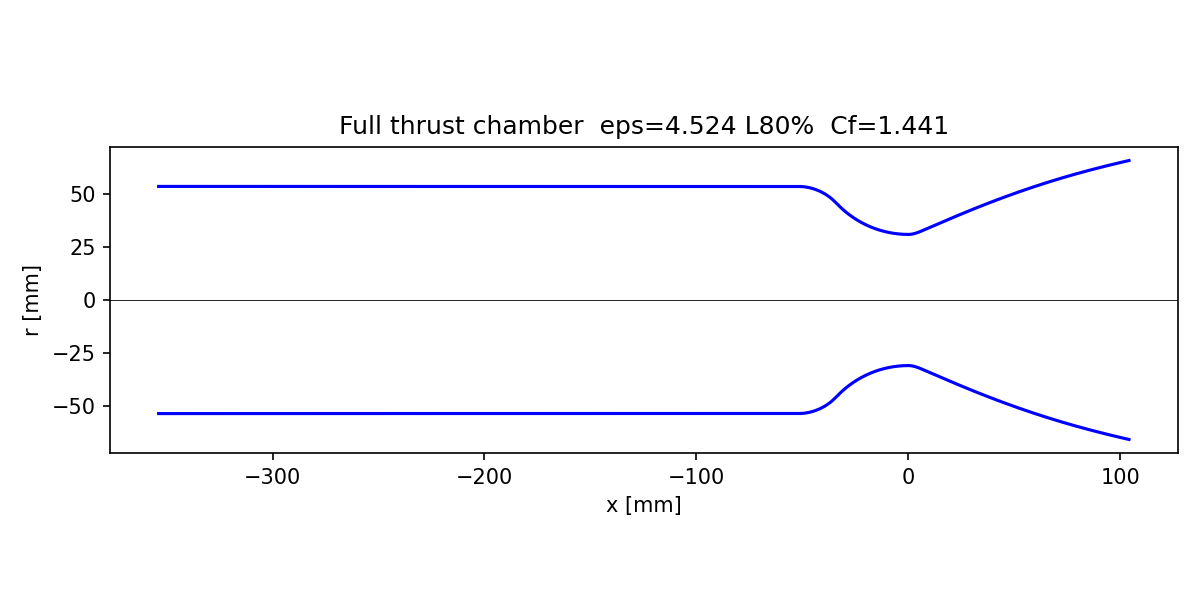
\includegraphics[width=\linewidth,trim=0 38 0 52,clip]{figures/fresh/fresh_13kn_chamber_contour_profile.png}
\caption{Fresh run (5 November): rao-bvp contour, $\varepsilon = 4.524$, 80\,\% bell, $C_F = 1.441$.}\label{fig:fresh-a}
\end{minipage}\hfill
\begin{minipage}[t]{0.315\linewidth}\centering
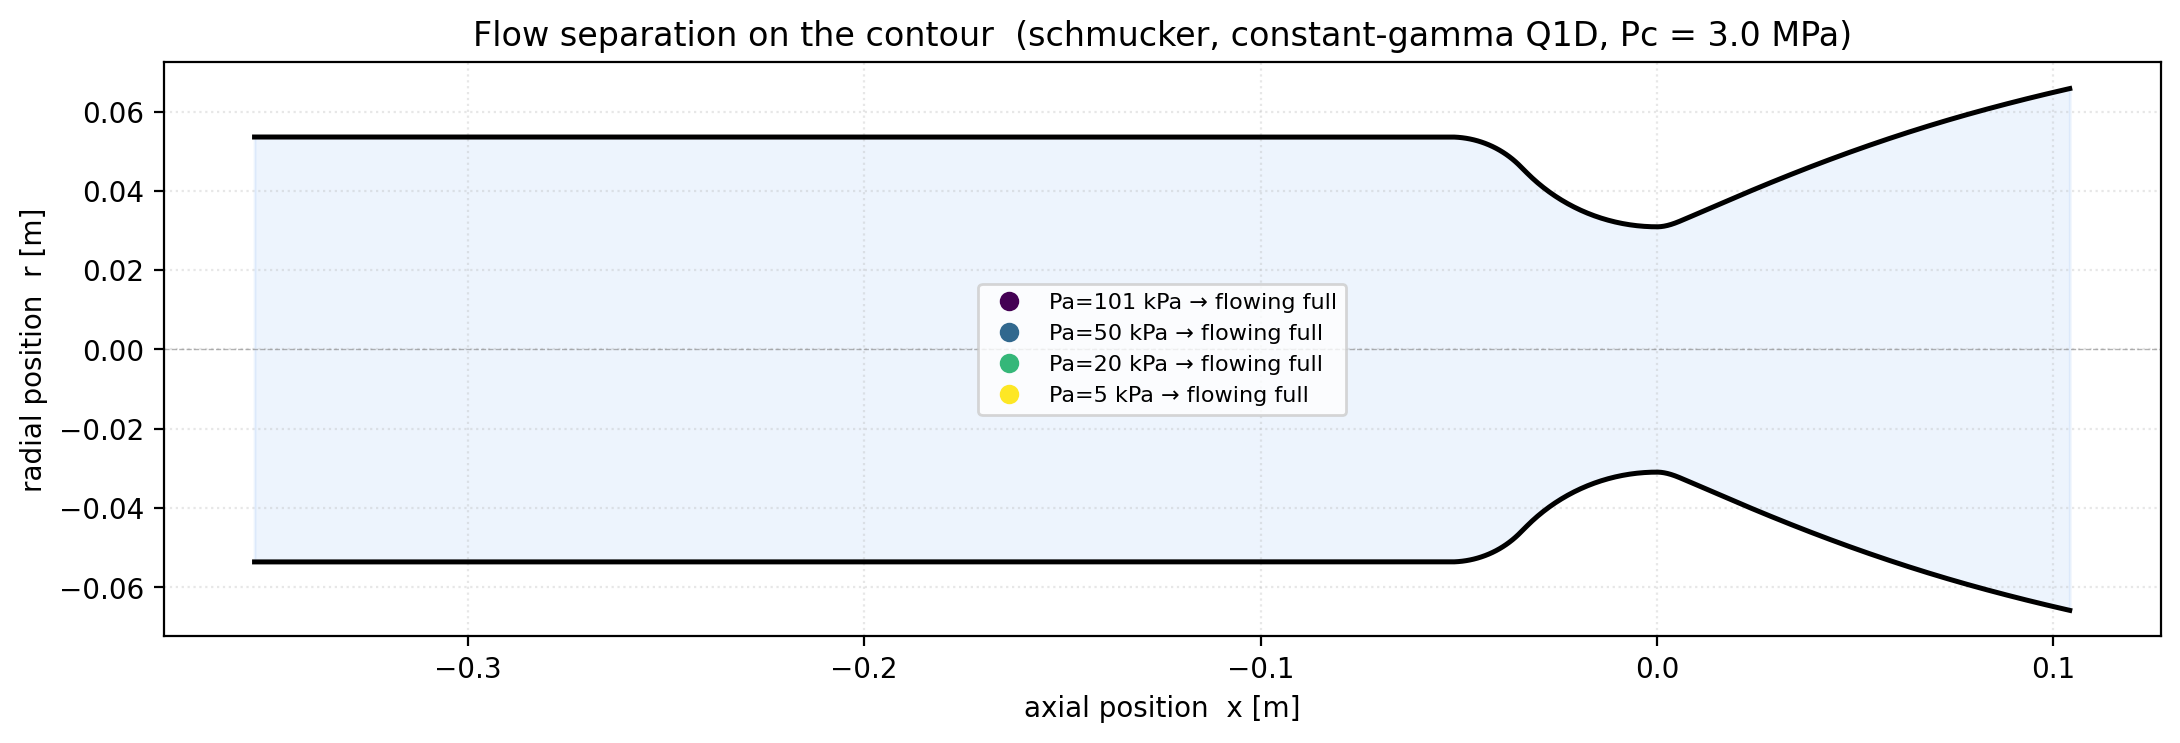
\includegraphics[width=\linewidth]{figures/fresh/fresh_13kn_separation_check_contour.png}
\caption{Fresh run: Schmucker separation screen, flowing full at 101, 50, 20 and 5 kPa.}\label{fig:fresh-b}
\end{minipage}\hfill
\begin{minipage}[t]{0.315\linewidth}\centering
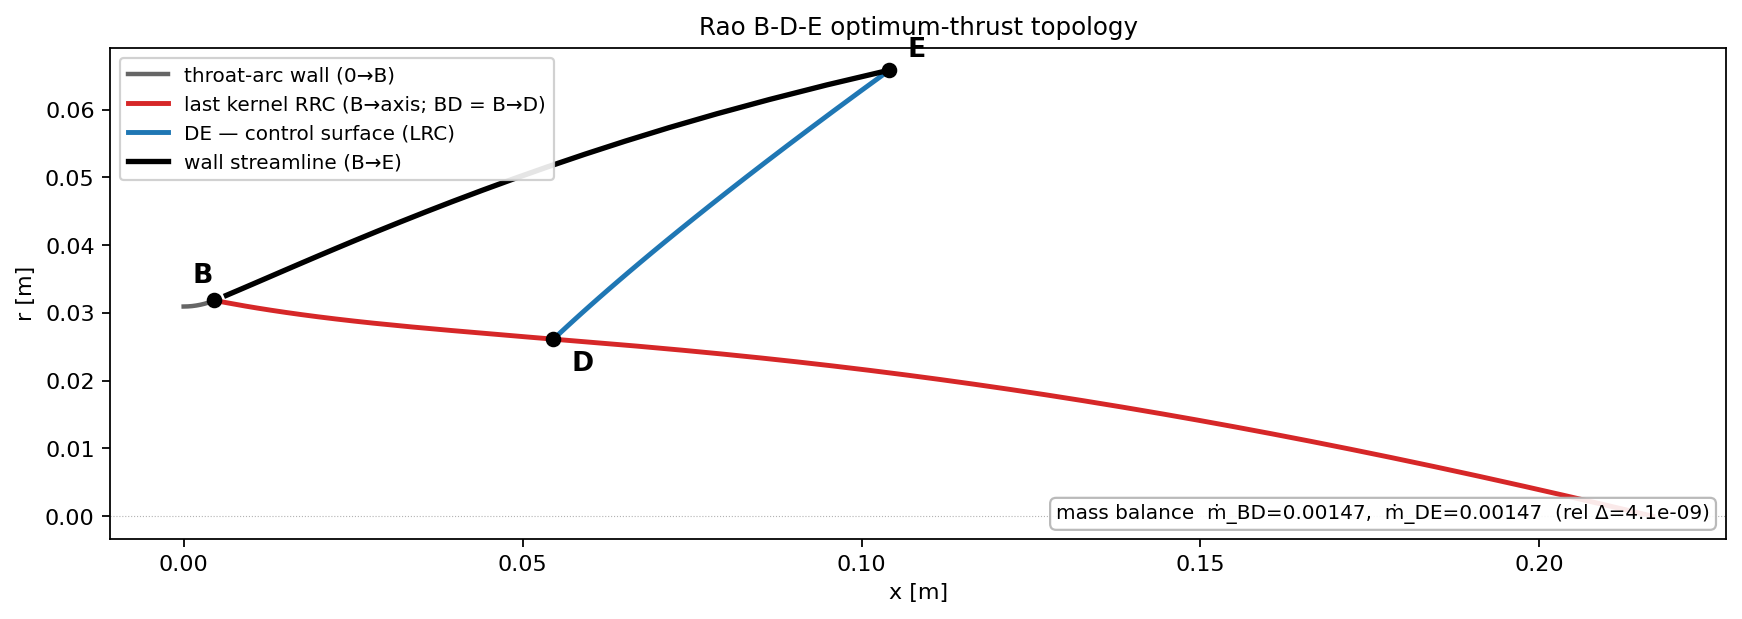
\includegraphics[width=\linewidth]{figures/fresh/fresh_13kn_rao_bde_topology.png}
\caption{Fresh run: Rao B-D-E topology; BD/DE mass balance relative difference $4.1\times10^{-9}$.}\label{fig:fresh-c}
\end{minipage}
\end{figure}

\begin{figure}[H]
\centering
\begin{minipage}[t]{0.315\linewidth}\centering
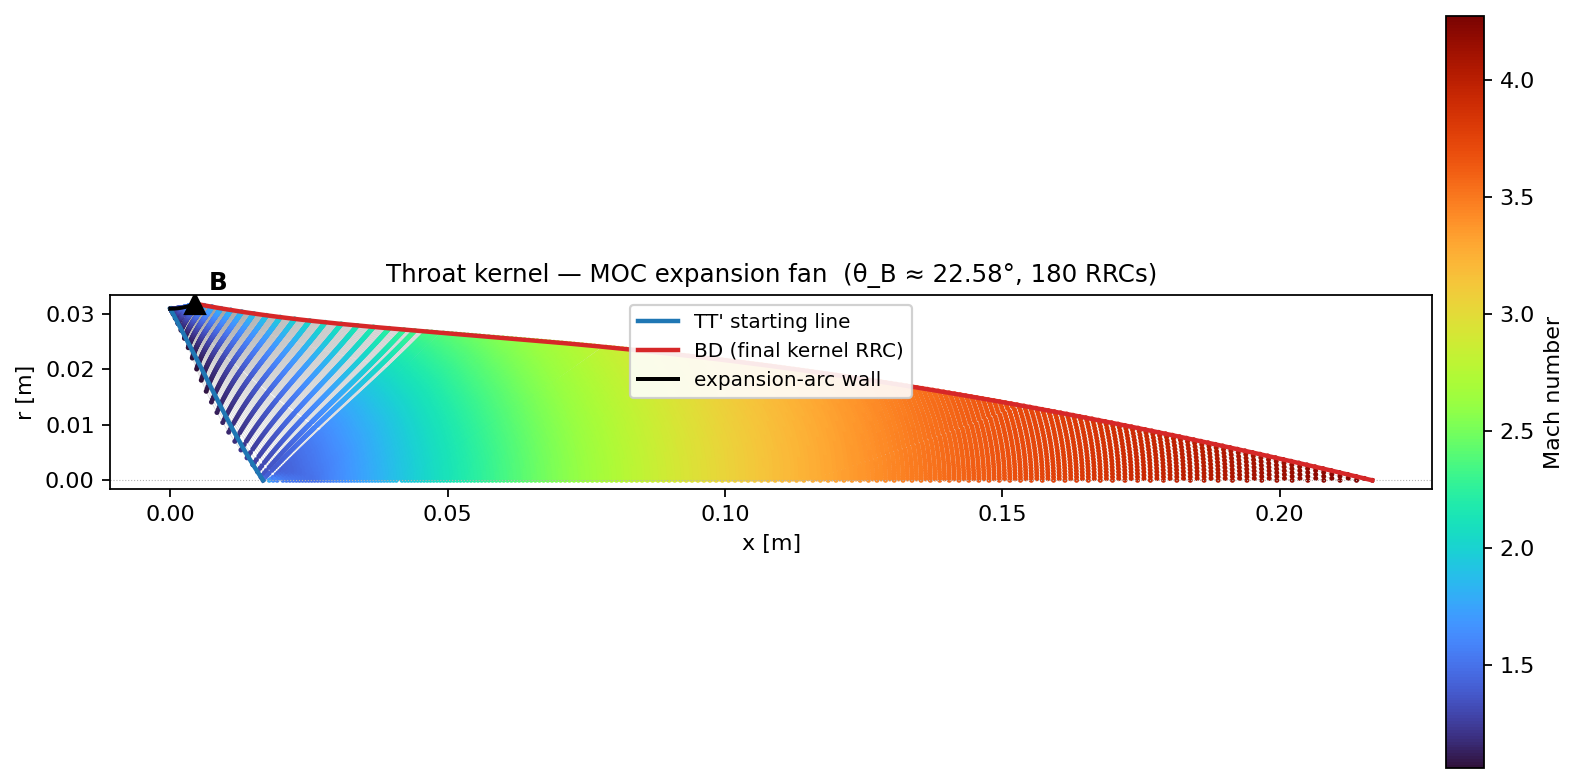
\includegraphics[width=\linewidth]{figures/fresh/fresh_13kn_throat_kernel_fan.png}
\caption{Fresh run: throat kernel with 180 RRCs (90 in July with the same arguments), $\theta_B \approx 22.58^\circ$.}\label{fig:fresh-d}
\end{minipage}\hfill
\begin{minipage}[t]{0.315\linewidth}\centering
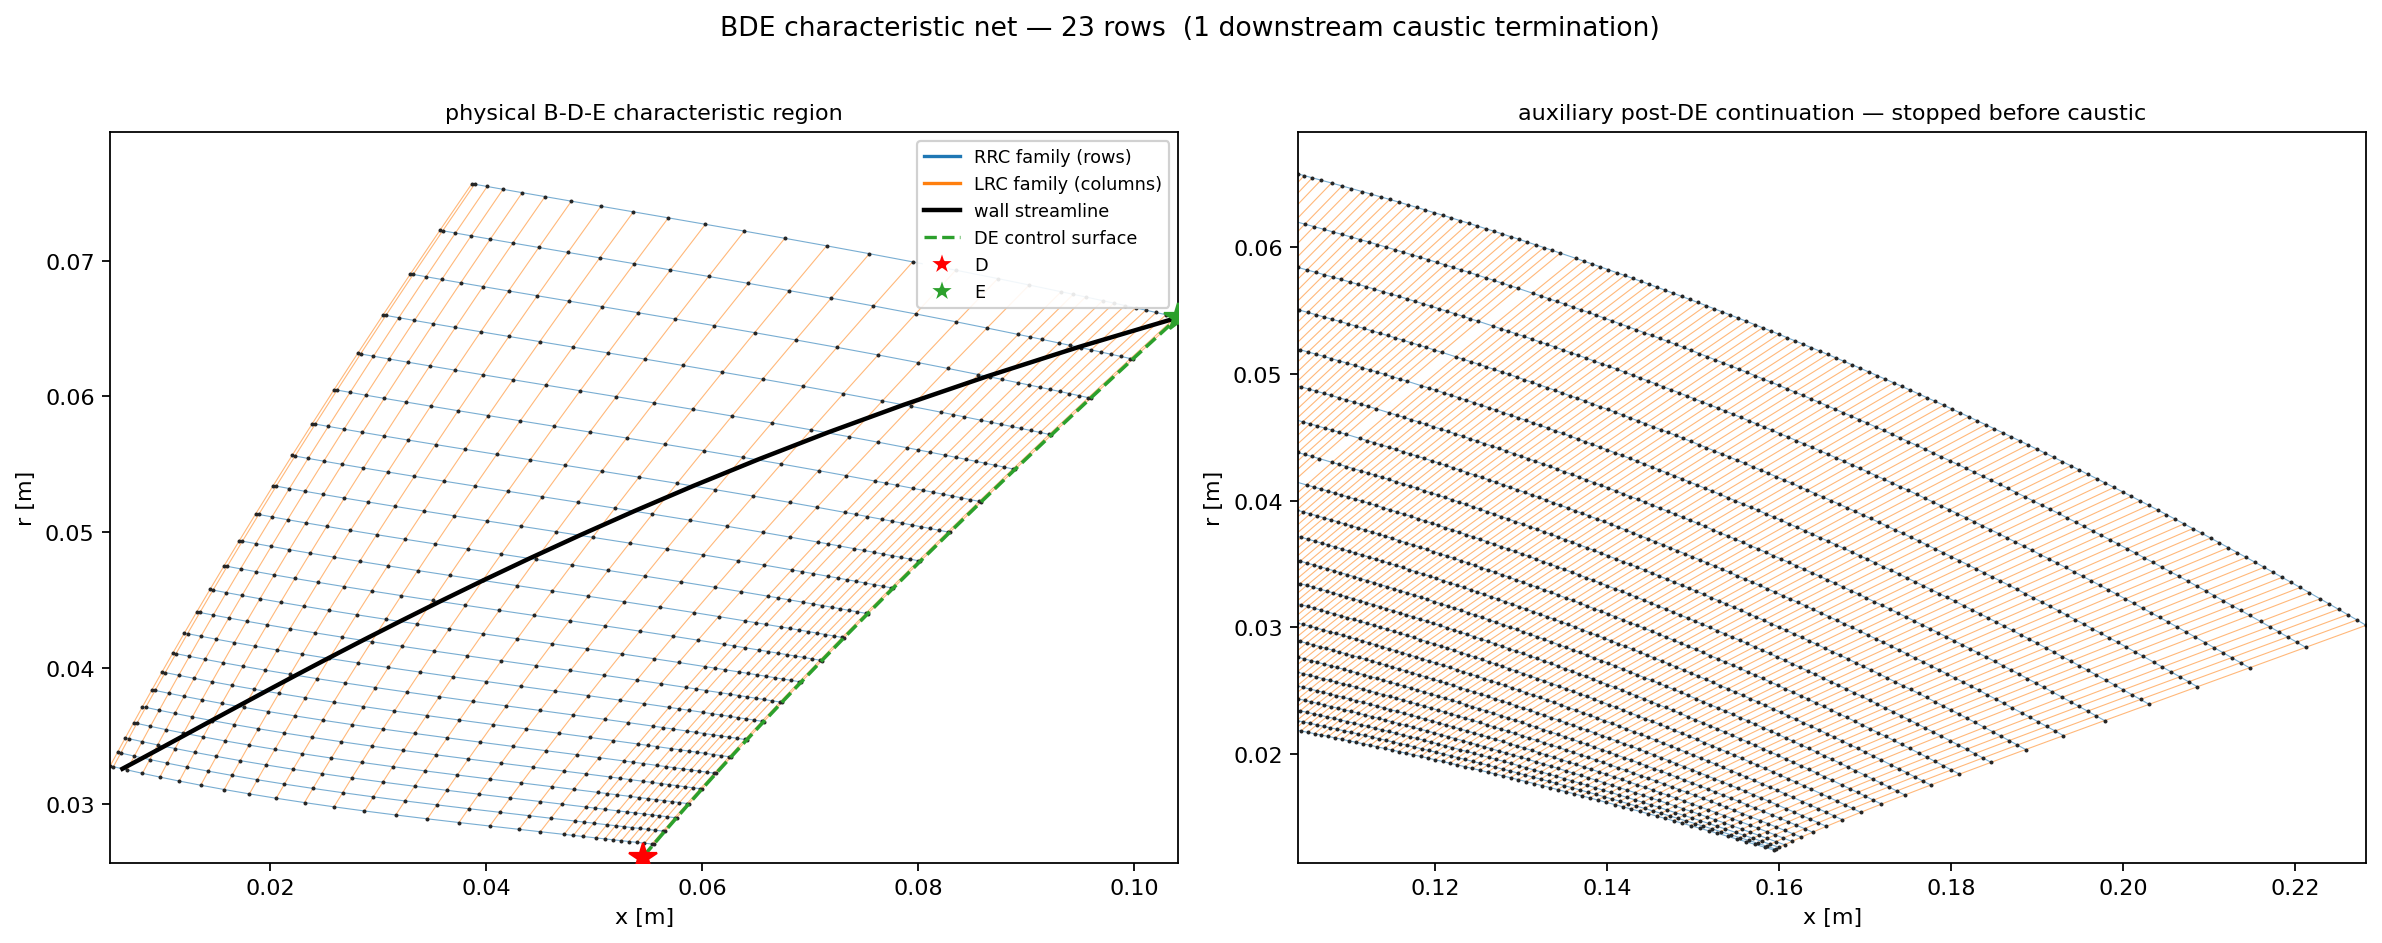
\includegraphics[width=\linewidth]{figures/fresh/fresh_13kn_bde_characteristic_net.png}
\caption{Fresh run: BDE net with 23 rows and one downstream caustic termination.}\label{fig:fresh-f}
\end{minipage}\hfill
\begin{minipage}[t]{0.315\linewidth}\centering
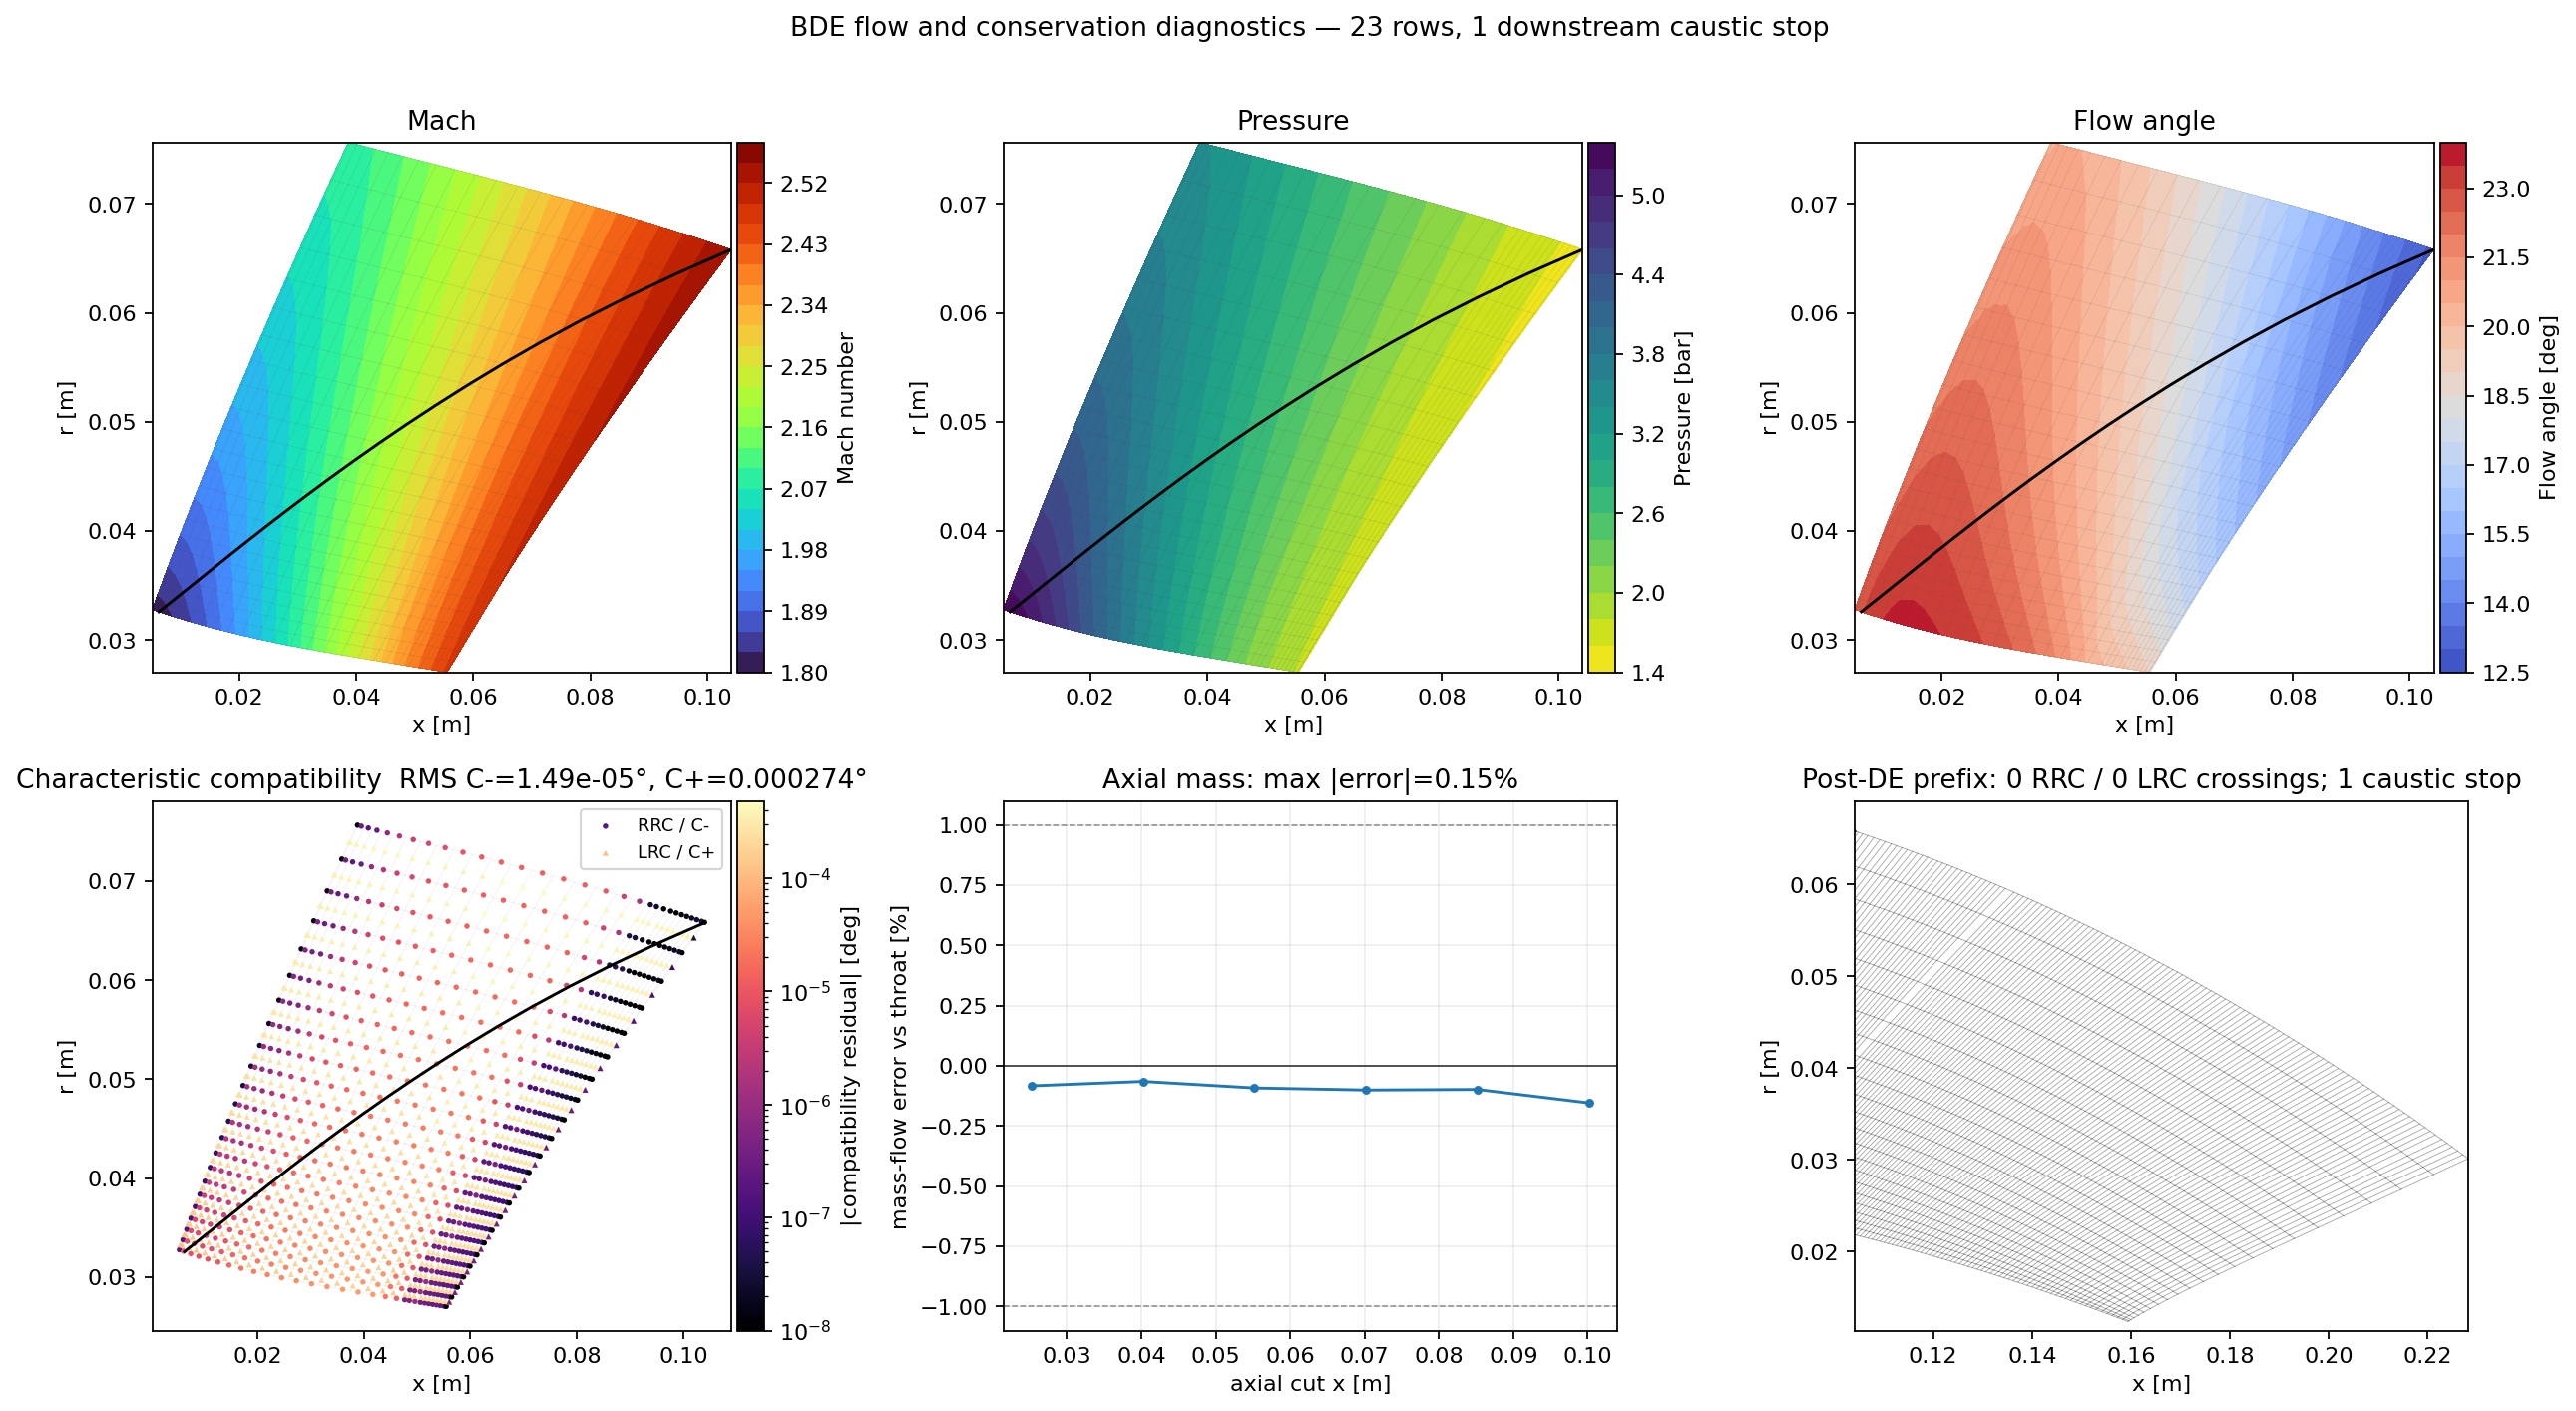
\includegraphics[width=\linewidth]{figures/fresh/fresh_13kn_bde_flow_conservation_diagnostics.png}
\caption{Fresh run: BDE diagnostics; compatibility RMS $1.49\times10^{-5}$ deg (C$^-$) and $2.74\times10^{-4}$ deg (C$^+$); axial mass error at most 0.15\,\%.}\label{fig:fresh-g}
\end{minipage}
\end{figure}

\begin{figure}[H]
\centering
\begin{minipage}[t]{0.315\linewidth}\centering
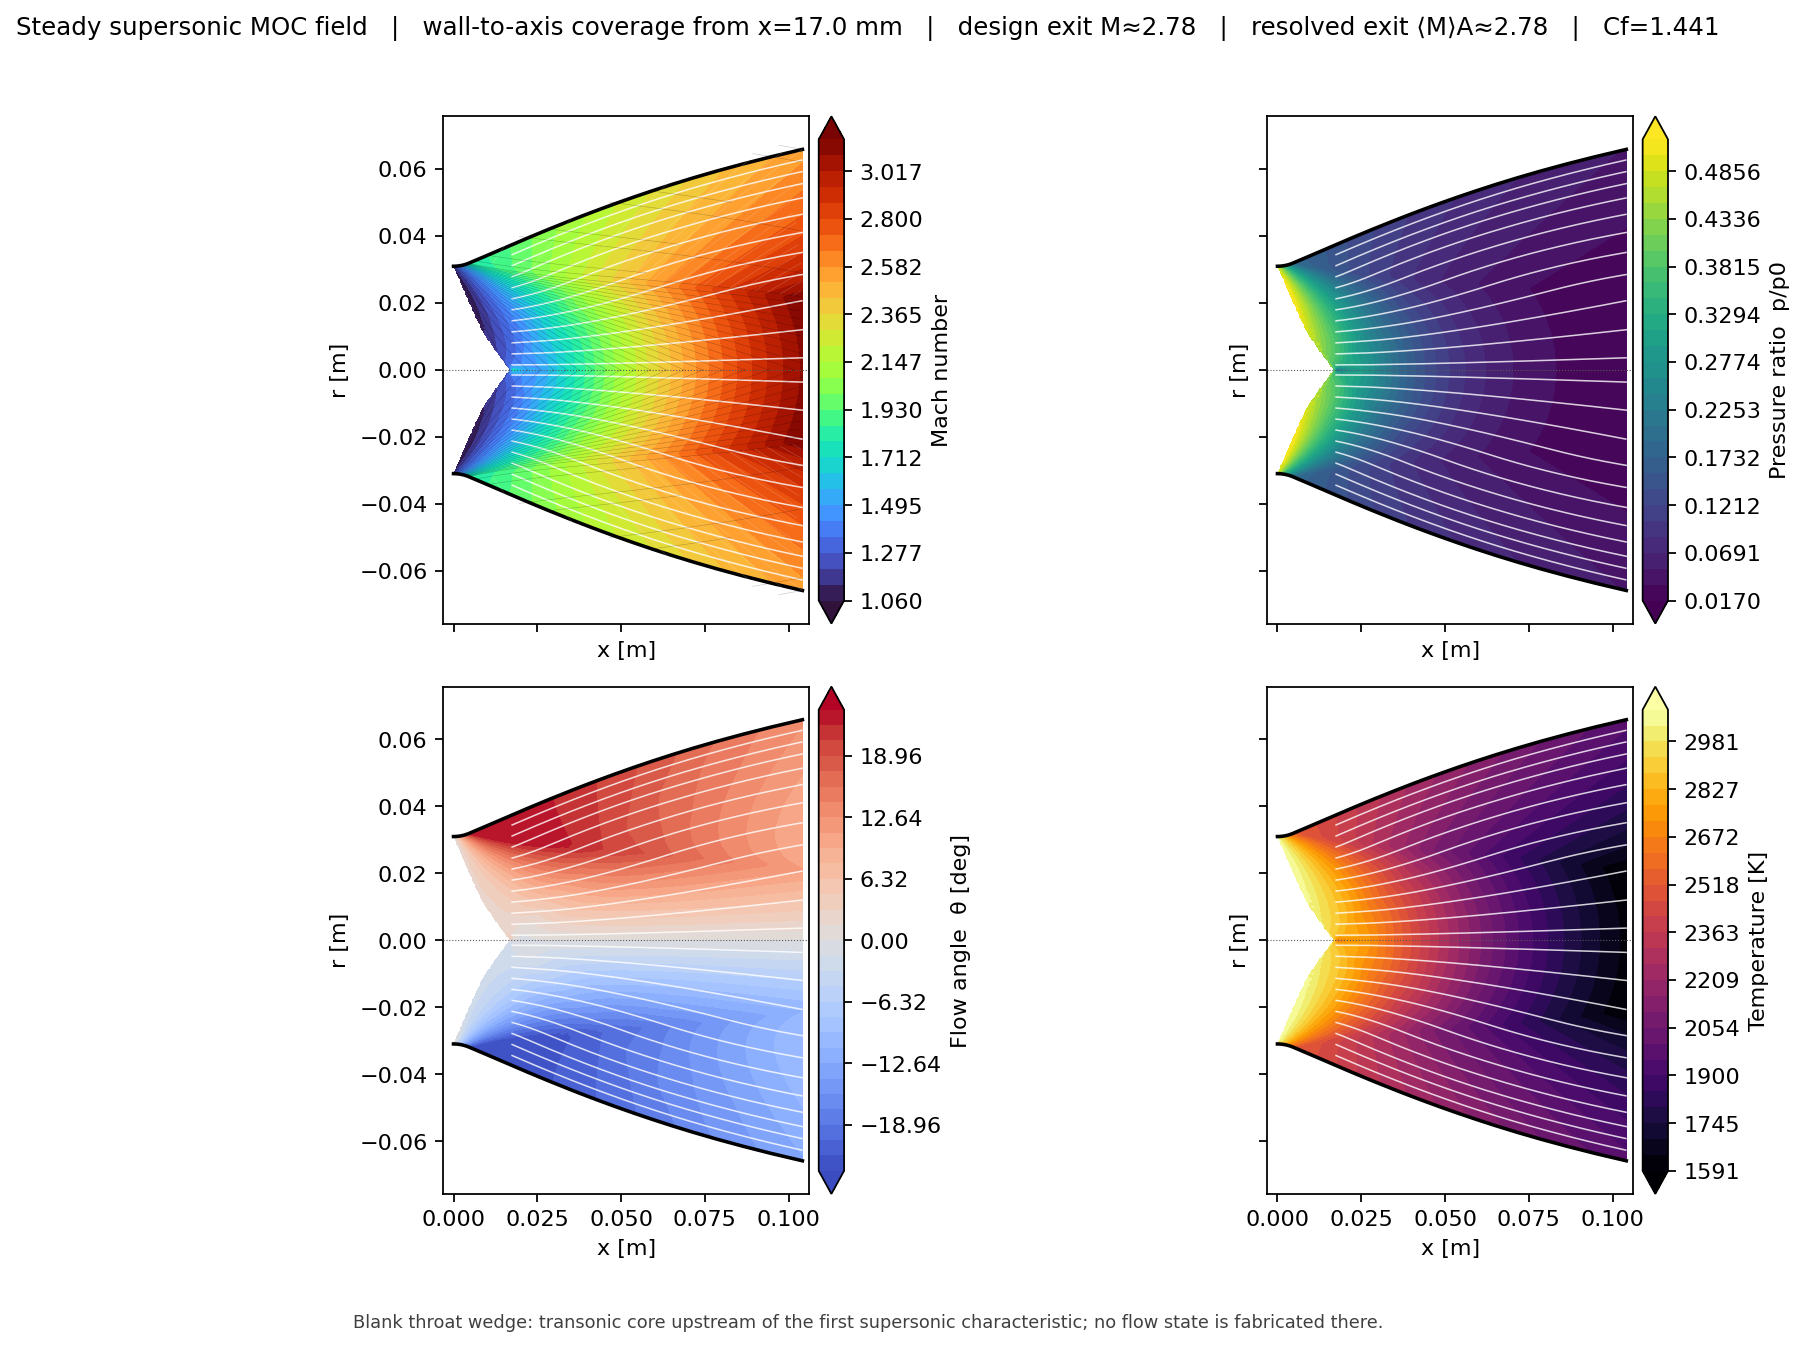
\includegraphics[width=\linewidth]{figures/fresh/fresh_13kn_moc_flowfield_mach_p_theta_T.png}
\caption{Fresh run: resolved MOC field (Mach number, $p/p_0$, flow angle, temperature); design and resolved exit Mach number 2.78.}\label{fig:fresh-e}
\end{minipage}\hfill
\begin{minipage}[t]{0.315\linewidth}\centering
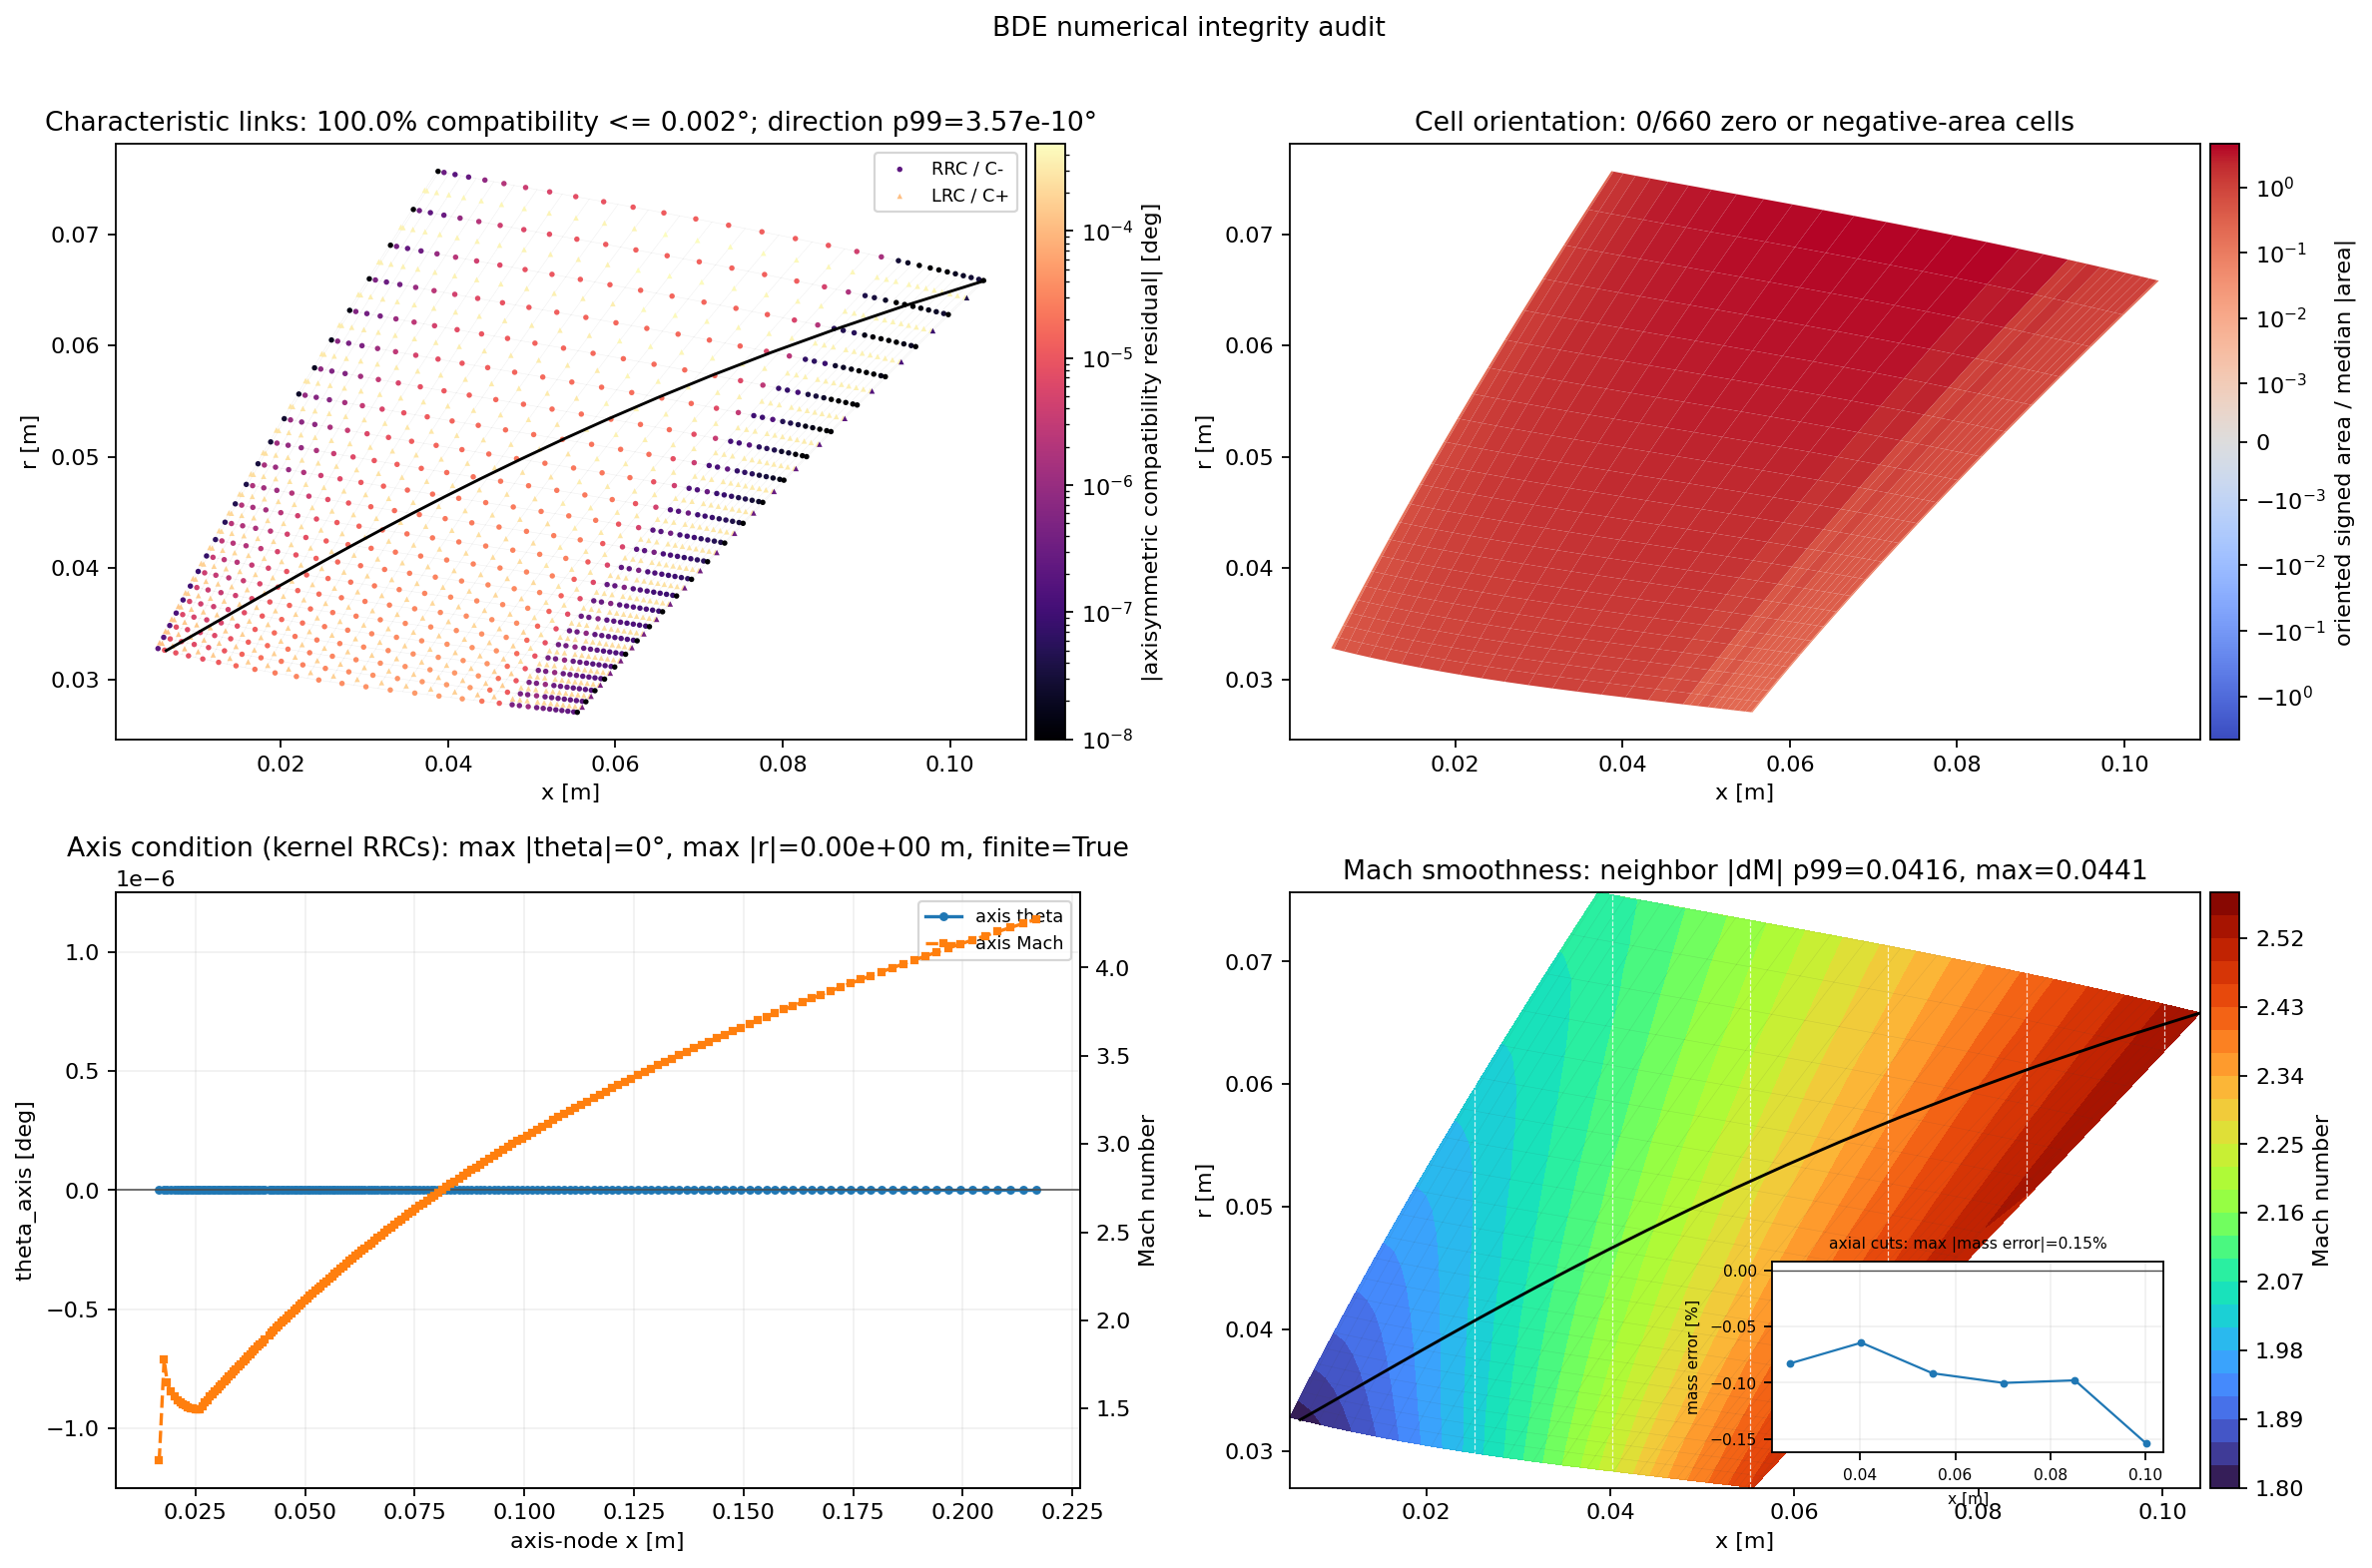
\includegraphics[width=\linewidth]{figures/fresh/fresh_13kn_bde_numerical_integrity_audit.png}
\caption{Fresh run: integrity audit; 0 of 660 cells degenerate; 99th-percentile neighbour Mach jump 0.042.}\label{fig:fresh-h}
\end{minipage}
\end{figure}

\subsection{What this says about the working tree}\label{sec:fresh-run-tree}

\caution{On the current working tree, the documented regression benchmark cannot run. Neither can any shipped example that uses the default Bezier/TOP contour with $\varepsilon < 5$. Only the opt-in rao-bvp path produces a contour at the 13\,kN sea-level point. Because the full-engine stages run after the contour, nothing in the regen, injector, pump or CAD stages could be exercised fresh. The newest evidence for those subsystems is still the July builds.}

\begin{enumerate}
\item \textbf{The chart change is incomplete.} The modified \code{raosim/nozzle_geometry.py} imports \code{raosim/rao_top_chart.py}, which \code{git} \code{status} lists as untracked (\code{??}). Committing the module without the new file would leave HEAD unable to import \code{nozzle_geometry}. The CLI-level override and its test were written for the old silent-extrapolation behaviour and were not updated (Section~\ref{sec:fresh-run-fail}).
\item \textbf{The benchmark documentation no longer matches the code.} Three statements are now wrong:
  \begin{itemize}
  \item The \code{.args} header says to append \code{--max-nfev} \code{0} for ``a quick seed-geometry smoke run''.
  \item \code{TEST_PROMPT.md} Step~1 says the file ``runs the full benchmark contour (\code{--max-nfev} \code{4000})''.
  \item \code{TEST_PROMPT.md} Step~5 says to expect ``minutes of runtime (JAX BVP solve)''.
  \end{itemize}
  The file selects the default Bezier path, whose build plan prints ``solver: not applicable (deterministic Rao/TOP chart geometry)''. The Bezier branch of \code{_solve} (\code{run_nozzle.py:1464-1487}) does not read \code{--max-nfev}, \code{--n-control} or \code{--n-kernel}, so the ``fast'' and ``full'' variants produce the same contour. The code is authoritative here. The 13 July \code{13kn_sl_full} summary already shows \code{contour_method:} \code{bezier} and \code{max_nfev:} \code{4000} recorded alongside \code{solver_gates_applicable:} \code{false}.
\item \textbf{The rao-bvp path is healthy and reproducible.} It runs end to end on the working tree and reproduces July's contour to solver tolerance, with denser construction diagnostics.
\item \textbf{The working tree is large and unsettled.} \code{git} \code{status} lists 18 modified modules under \code{raosim/} and the untracked \code{raosim/rao_top_chart.py}, \code{raosim/thermal_correlations.py} and \code{raosim/data/}. Across the tree, \code{git} \code{diff} \code{--stat} reports 153 files changed, most of them documentation moves. Any build made from this tree describes a state that no commit contains.
\end{enumerate}

%======================================================================
\section{Known defects visible in the builds}\label{sec:build-defects}

Each item below is visible in a build or in today's run. The status is as of 5 November 2026. Where a cause is given, it was found by reading the current code, and no fix was attempted.

\begin{enumerate}[leftmargin=1.9em]
\item \textbf{The default contour path rejects the shipped benchmark.} Covered in Section~\ref{sec:fresh-run}. Current, and it blocks Step~1 of \code{TEST_PROMPT.md}.

\item \textbf{\code{13kn_sl_full} records \code{pump_package:} \code{failed} with \code{KeyError:} \code{'valid'}.} This is not the 13 July sandbox's bolt-sector failure. The sandbox report (written 15:49) records that fix the same day. \code{13kn_sl_full} was written later, at 17:22--17:23, and every fuel and oxidizer B-rep part in its \code{pump/pump_brep/} carries those timestamps, including \code{oxidizer_volute_body} and \code{oxidizer_volute_front_cover}. The split casing was therefore built.

The failure comes afterwards, when the summary is assembled. \code{raosim/pump_cad_brep.py} (lines 1486--1492) stores the split-casing bolt layout in the per-role diagnostics dictionary as \code{<role>_split_casing_layout}. That entry is a geometry dictionary with keys such as \code{flange_outer_radius_mm} and \code{bolt_hole_radius_mm}, and it has no \code{valid} key. \code{raosim/run_nozzle.py} (lines 6275--6281) then reads \code{info["valid"]} for every diagnostics entry. The broad \code{except} at line 6313 catches the resulting \code{KeyError} and records \code{pump_package} with \code{status:} \code{failed}. The \code{pump_package.brep_diagnostics} check required by \code{TEST_PROMPT.md} Step~2 can therefore not pass whenever a volute is built. Neither file has a functional change since HEAD (the only working-tree edit to \code{run_nozzle.py} is a documentation path in a help string), so the defect is current. No test refers to \code{split_casing_layout} or \code{brep_diagnostics}.

\item \textbf{The \code{13kn_sl_fast} contour is seed-only.} The summary reports \code{seed_only:} \code{true}, \code{max_scaled} $2.32\times10^{-3}$ against a $2\times10^{-3}$ gate and \code{optimization_converged:} \code{false}. Its top-level \code{Cf} of 1.0747 is not a performance figure; the performance block gives 1.441. The thermal, injector and pump results are built on this unconverged wall, and today the same command cannot produce a seed contour at all (Section~\ref{sec:fresh-run-tree}).

\item \textbf{Some directories mix dates.} \code{13kn_sl_full} combines two runs:
  \begin{itemize}
  \item From 13 July: \code{summary.json}, \code{contour.csv}, the cooling and structural PNGs and the pump package.
  \item From 3 July: \code{wall.stl}, \code{jacket.stl}, \code{regen.stl}, \code{regen_3d.png}, the injector PNGs, the construction diagrams \code{kernel_fan.png}, \code{rao_topology.png} and \code{bde_mesh.png}, the whole \code{pintle/} tree and the two \code{*_volute_casing} files.
  \end{itemize}
  The 13 July summary has no \code{wall_geometry} or \code{regen} block, so it does not describe the STLs beside it. Its contour is Bezier, while the MOC construction diagrams beside it can only come from an earlier BVP run. Its \code{pintle/} folder holds both the superseded three-part STEP files (\code{pintle_post_slotted}, \code{annular_sleeve}, \code{injector_face_machined}) and the five-part coaxial set. \code{13kn_sl_fast} also contains five pintle-part STLs from 2 July.

\item \textbf{Single summaries contradict themselves.} \code{13kn_sl_fast} carries three channel heights, two coolant pressure drops and two $\eta_{c^*}$ values (Sections~\ref{sec:builds-pic-regen} and~\ref{sec:builds-pic-injector}). The chamber length the injector uses also differs between builds: 0.3017\,m (the cylinder) in \code{13kn_sl_fast} and 0.3538\,m (face to throat) in \code{13kn_sl_full}.

\item \textbf{The test suite writes into \code{builds/}.} \code{tests/test_design_workflow.py} line 181 runs \code{main.py} from the repository root and leaves three versioned builds per run. This produced the 436-build \code{versioned-cli-contour} family and, on the archive day, v455--v463 (07:03 to 07:18).

\item \textbf{Builds cannot be reproduced.} No build stores its command line, there is no run log next to most builds, and the baseline file for \code{TEST_PROMPT.md} Step~4 has never existed. Drift against a known reference can only be judged by hand against the 2 July snapshot numbers quoted in \code{TEST_PROMPT.md}, which \code{13kn_sl_fast} reproduces.

\item \textbf{The legacy \code{main.py} MOC and Rao methods fail in every run.} Since May, every \code{moc} build reports \code{nan} exit Mach number and exit angle, and every \code{rao} build reports $\theta_e = 88.16^\circ$ with \code{method_status} failing (Table~\ref{tab:builds-vnnn}). These are the legacy toolbox methods. The main CLI's bounded MOC net and the rao-bvp solver are separate code.

\item \textbf{Documentation lags the code.} Besides the \code{.args} header and \code{TEST_PROMPT.md} (Section~\ref{sec:fresh-run-tree}), the sandbox report's host follow-up promises that the ``full 4000-nfev JAX solve \dots{} also produces the MOC construction diagrams''. The code refuses \code{--flowfield} on the Bezier path (\code{run_nozzle.py:3900-3904}). \code{examples/cli/} has no \code{README}.
\end{enumerate}

\decision{\textbf{Where the app stands.}
\begin{itemize}
\item The most complete coherent engine package is \code{13kn_sl_fast} from 8 July. It covers station-wise regen sizing, structural and life screens, the pintle injector and feed gates, meanline electric pumps and valid pump B-rep parts, all on a seed-only contour.
\item The best contour and flow-field evidence is the rao-bvp run, first on 17 July and reproduced on 5 November.
\item On 5 November the default Bezier/TOP path cannot run the shipped 13\,kN benchmark, because of an uncommitted, partly tracked chart change.
\item The \code{KeyError} in pump summary assembly still means that a complete pump B-rep package is recorded as failed.
\item Every result is preliminary or experimental by the repository's own labels; \code{hardware_qualified} is false throughout, and 17 external-evidence items block physical release.
\end{itemize}}
